
\chapter{Neural Radiance Caching}
\label{chap:nrc}
\begin{figure}[htb!]
    \centering
    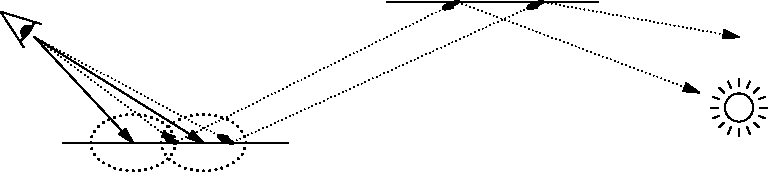
\includegraphics{figures/asy/nrc.pdf}
    \caption{Visualization of radiance caching. Full paths (dotted arrows) are only evaluated sparsely, and their radiance estimates are cached per vertex (small arrows). To render the image, short paths (solid arrows) are traced from the camera to collect cached radiance by interpolation (dotted circles).}
    \label{fig:nrc_overview}
\end{figure}
A weak point of the reference Monte Carlo pathtracer motivated in \cref{chap:pathtracing} is, that we have to start from zero, every time the scene or camera changes.
It would make sense to keep samples around that can be reused when temporally and spatially similar paths occur in the evaluation of the global illumination integral.
Radiance caching by \textcite{ward1988} addresses this problem by caching sparse estimates of the radiance field.
To generate full resolution images, radiance is interpolated from cached estimates.

A particularly interesting variant of radiance caching is Neural Radiance Caching (NRC) by \textcite{muller2021}.
They train a neural network to predict the radiance along training paths generated using path tracing.
For inference, they then replace the recursive path tracing integral with a neural estimate of the radiance field when the variance along the path becomes too high.
The Neural Radiance Cache can be interpreted as a classical cache that uses gradient descent for temporally smooth cache updates and the generalization capabilities of neural networks to interpolate between cached samples.
Furthermore, this approach could also be viewed as a form of path space denoising of the radiance field.

\textcite{dereviannykh2024} recently adapted the NRC to predict \emph{incident} radiance instead.
Yet, this is probably not well suited for the caustics' problem this thesis aims to solve, which exhibit high-frequency sparse incident radiance but low-frequency dense outgoing radiance.
Thus, this thesis only explores classical NRC, although applying the radiance estimators from \cref{chap:bidirectional_caching} to the Neural Incident Radiance Cache (NIRC) may pose an interesting topic for future research.

\section{Network Architecture}
\label{sec:fully_fused}
Because the network has to be trained and evaluated in real-time, \textcite{muller2021,muller2022} propose to use a rather small hardware-accelerated network architecture.
They use a fully connected network with 3-5 hidden layers, depending on the input encoding, with 64 neurons and ReLU activation functions each.
The output layer has 3 values, one for each color channel.
Additionally, they omit biases as they did not observe a measurable benefit and it simplifies the implementation.
Because of the shallow architecture, skip connections are not needed to preserve the gradient flow.

To maximize the inference and training performance, \textcite{muller2021} introduce a fully fused implementation of the network, which fully utilizes shared memory and per-thread registers.
For this, the whole network is implemented as a single CUDA kernel, with each block handling a batch of 128 64-dimensional input vectors and keeping the $64\times128$ activations in shared memory.
Each block then consists of 4 warps, computing 16 neuron activations each by applying a $16\times64$ matrix multiplication and the element-wise activation function.
For this, the hardware accelerated $16\times16$ FP16 matrix multiplication instruction is used when available.
With this hardware-optimized implementation, \textcite{muller2021} achieve a speedup of $5\times$ to $10\times$ compared to the widely used TensorFlow framework \parencite{tensorflowdevelopers2021} on large batch sizes corresponding to HD resolution.

\section{Input Encodings}
\begin{table}[htb!]
    \centering
    \begin{tabular}{l l l}
        %\toprule
        \textbf{Parameter} & \textbf{Encoding} & \textbf{Dimensions} \\
        \midrule
        Position $\vec{x} \in \mathbb{R}^3$ & $\mathrm{mhe}(\vec{x}) \in \mathbb{R}^{16 \times 2}$ & 0--31 \\
        Direction $\wo \in \mathbb{S}^2$ & $\mathrm{ob}(\wo) \in \mathbb{R}^{2 \times 4}$ & 32--39 \\
        Normal $\vec{n}(\vec{x}) \in \mathbb{S}^2$ & $\mathrm{ob}(\vec{n}(\vec{x})) \in \mathbb{R}^{2 \times 4}$ & 40--47 \\
        Roughness $r(\vec{x}) \in [0,1]$ & $\mathrm{ob}(r(\vec{x})) \in \mathbb{R}^{4}$ & 48--51 \\
        Diffuse reflectance $\vec{F}_d(\vec{x}, \wo) \in [0,1]^3$ & $\vec{F}_d(\vec{x}, \wo) \in \mathbb{R}^{3}$ & 51--53 \\
        Specular reflectance $\vec{F}_s(\vec{x}, \wo) \in [0,1]^3$ & $\vec{F}_s(\vec{x}, \wo) \in \mathbb{R}^{3}$ & 54--57 \\
        Padding $\vec{1} \in \mathbb{R}^7$ & $\vec{1} \in \mathbb{R}^7$ & 57--63 \\ % TODO: Check implementation
        %\bottomrule
    \end{tabular}
    \caption{The components of the 64-dimensional input vector to the neural network.}
    \label{tab:input-encoding}
\end{table}
As shown by \textcite{ren2013}, parametrizing the network with the outgoing direction $\wo$ and the position $\vec{x}$ alone is not sufficient for an accurate representation of the radiance field.
Instead, it proves beneficial to include the surface normal $\vec{n}$, surface roughness $r$ and the expected diffuse and specular reflectance terms $\vec{F}_d$ and $\vec{F}_s$ as well.
The diffuse reflectance $\vec{F}_d$ is simply the diffuse albedo for Lambertian surfaces.
To compute the specular reflectance $\vec{F}_s$, we have to compute the integral over the hemisphere of incoming directions in a white furnace environment.
Fortunately, this can be efficiently precomputed by generating a lookup table over the roughness and the cosine of the viewing angle that stores both a bias and a scaling factor on the Fresnel reflectance at normal incidence $\vec{F}_0$ (see \cref{fig:lut}).
The formula and derivation is given by \textcite{karis2013}, who use the specular reflectance to filter environment maps for approximate image-based lighting.
\begin{figure}[htb!]
    \centering
    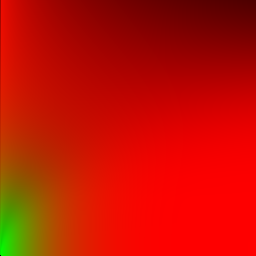
\includegraphics[width=0.15\textwidth]{figures/lut.png}
    \caption{Lookup table for the specular reflectance $\vec{F}_s$. The x-axis is the cosine of the viewing angle, and the y-axis is the roughness. The red channel gives the scaling factor on $\vec{F}_0$, the green channel the additional constant term.}
    \label{fig:lut}
\end{figure}

Furthermore, the correlation between the outgoing radiance and the input features $\vec{x}$, $\wo$, $\vec{n}$ and $r$ is highly non-linear, so additional effort is required to linearize the input space, as neural networks approximate (roughly) linear functions more efficiently.
The diffuse and specular reflectance on the other hand can be used directly, as the outgoing radiance will essentially be a linear combination of these two terms.

\subsection{Positional Encodings}

\paragraph{Triangle Wave Encoding}
A natural idea to linearize the input space is to find a set of orthonormal basis functions.
This enables the neural network to approximate arbitrarily complex functions on the input space as a linear combination of these basis functions.
A very famous such basis set is the Fourier series, which forms a basis for the space of square-integrable functions on the interval $[0, 1]$.
Square-integrability is not really a constraint, as it essentially assumes finite energy, which is a reasonable assumption to make for the radiance field.
Neither is the limitation to $[0, 1]$, as we can always normalize the input to the bounding box of the scene.
Such types of encodings were first used in language processing by \textcite{vaswani2017} and later adapted to computer graphics by \textcite{tancik2020} and to neural radiance fields by \textcite{mildenhall2020}.

However, for practical applications, compromises are necessary:
Firstly, \textcite{tancik2020} make the assumption that the output field is separable in the input dimensions, which is generally not the case, resulting in stripe artifacts in the output if the network is too shallow to adequately mitigate this nonlinearity.
Yet, this allows them to apply the Fourier transform individually per input dimension and brings the number of coefficients down from exponential to linear in the number of dimensions.
The hope is, that the neural network can compensate for the missing information.
This is generally possible, as every non-separable function can be approximated by a linear combination of separable functions, for example by writing the function as a tensor and applying tensor decomposition.
Additionally, \textcite{muller2021} omit the cosine terms and approximate the sine terms with triangle waves, which they found to reduce the number of coefficients and the computational cost without visibly affecting the output quality.

\paragraph{Instant Neural Graphic Primitives}
In a follow-up work, \textcite{muller2022} propose a new positional encoding scheme, which they call Multiresolution Hash Encoding (MHE).
The idea is, to distribute feature vectors in a hierarchical grid in space.
For a given input position $\vec{x}$ and for each grid level a feature vector is then obtained by linearly interpolating the feature vectors at the corners of the current grid cell.
The individual feature vectors are concatenated and used as input to the neural network.
During training, the gradient is propagated back to the feature vectors.
To reduce the size of the backing feature grid and to better represent sparse fields, \textcite{muller2022} use a hash table per grid level.
For the hyperparametrization of the grid, \textcite{muller2022} empirically found 16 levels with 2 features per grid level to be Pareto optimal for their applications, which is adopted here as well.

\subsection{Directional Encodings}

\paragraph{Spherical Harmonics}
A popular choice for the encoding of direction vectors is the use of spherical harmonics.
This is a natural choice, as the spherical harmonics form an orthonormal basis for the space of square-integrable functions defined on the unit sphere, so every function on directions can be represented as a linear combination of spherical harmonics, whose coefficients can be learned by the neural network.
However, the number of basis functions is quadratic in the degree $m$, which limits us to a maximum degree of $m=3$ for the 64-dimensional input vector, and they are relatively expensive to compute.
The limited degree also hinders the representation of high-frequency details in the radiance field.
Thus, it is worth-while to also explore alternative encodings for $\wo$ and $\vec{n}$.

\paragraph{One Blob and One Blob Diffuse Encoding}
For bounded domains, \textcite{muller2019} propose a simple encoding scheme, which is a continuous generalization of the popular one-hot encoding, they call One Blob Encoding.
The idea is, to divide the input space into a fixed number of bins along each dimension.
Each input vector is then assumed to be distributed over the bins by a Gaussian distribution and the activation of the bin is the probability of the input vector to fall into that bin.
This probability is simply the integral of the PDF over the bin, which can be computed using the cumulative distribution function (CDF):
\begin{equation}
    \mathrm{ob}(x)_i = \probability{b_i \leq x < b_{i+1}} = \probability{x < b_{i+1}} - \probability{x < b_i},
\end{equation}
where $b_i$ and $b_{i+1}$ are the boundaries of the $i$-th bin.
To improve performance, \textcite{muller2021} approximate the Gaussian distribution with a fourth order polynomial (see \cref{fig:oneblob}).

\begin{figure}[htb!]
    \centering
    \begin{subfigure}{0.5\textwidth}
        \centering
        %% Creator: Matplotlib, PGF backend
%%
%% To include the figure in your LaTeX document, write
%%   \input{<filename>.pgf}
%%
%% Make sure the required packages are loaded in your preamble
%%   \usepackage{pgf}
%%
%% Also ensure that all the required font packages are loaded; for instance,
%% the lmodern package is sometimes necessary when using math font.
%%   \usepackage{lmodern}
%%
%% Figures using additional raster images can only be included by \input if
%% they are in the same directory as the main LaTeX file. For loading figures
%% from other directories you can use the `import` package
%%   \usepackage{import}
%%
%% and then include the figures with
%%   \import{<path to file>}{<filename>.pgf}
%%
%% Matplotlib used the following preamble
%%   \def\mathdefault#1{#1}
%%   \everymath=\expandafter{\the\everymath\displaystyle}
%%   \IfFileExists{scrextend.sty}{
%%     \usepackage[fontsize=10.000000pt]{scrextend}
%%   }{
%%     \renewcommand{\normalsize}{\fontsize{10.000000}{12.000000}\selectfont}
%%     \normalsize
%%   }
%%   
%%   \ifdefined\pdftexversion\else  % non-pdftex case.
%%     \usepackage{fontspec}
%%     \setmainfont{DejaVuSerif.ttf}[Path=\detokenize{/opt/homebrew/Cellar/python-matplotlib/3.10.3/libexec/lib/python3.13/site-packages/matplotlib/mpl-data/fonts/ttf/}]
%%     \setsansfont{DejaVuSans.ttf}[Path=\detokenize{/opt/homebrew/Cellar/python-matplotlib/3.10.3/libexec/lib/python3.13/site-packages/matplotlib/mpl-data/fonts/ttf/}]
%%     \setmonofont{DejaVuSansMono.ttf}[Path=\detokenize{/opt/homebrew/Cellar/python-matplotlib/3.10.3/libexec/lib/python3.13/site-packages/matplotlib/mpl-data/fonts/ttf/}]
%%   \fi
%%   \makeatletter\@ifpackageloaded{underscore}{}{\usepackage[strings]{underscore}}\makeatother
%%
\begingroup%
\makeatletter%
\begin{pgfpicture}%
\pgfpathrectangle{\pgfpointorigin}{\pgfqpoint{4.539660in}{3.141564in}}%
\pgfusepath{use as bounding box, clip}%
\begin{pgfscope}%
\pgfsetbuttcap%
\pgfsetmiterjoin%
\definecolor{currentfill}{rgb}{1.000000,1.000000,1.000000}%
\pgfsetfillcolor{currentfill}%
\pgfsetlinewidth{0.000000pt}%
\definecolor{currentstroke}{rgb}{1.000000,1.000000,1.000000}%
\pgfsetstrokecolor{currentstroke}%
\pgfsetdash{}{0pt}%
\pgfpathmoveto{\pgfqpoint{0.000000in}{0.000000in}}%
\pgfpathlineto{\pgfqpoint{4.539660in}{0.000000in}}%
\pgfpathlineto{\pgfqpoint{4.539660in}{3.141564in}}%
\pgfpathlineto{\pgfqpoint{0.000000in}{3.141564in}}%
\pgfpathlineto{\pgfqpoint{0.000000in}{0.000000in}}%
\pgfpathclose%
\pgfusepath{fill}%
\end{pgfscope}%
\begin{pgfscope}%
\pgfsetbuttcap%
\pgfsetmiterjoin%
\definecolor{currentfill}{rgb}{1.000000,1.000000,1.000000}%
\pgfsetfillcolor{currentfill}%
\pgfsetlinewidth{0.000000pt}%
\definecolor{currentstroke}{rgb}{0.000000,0.000000,0.000000}%
\pgfsetstrokecolor{currentstroke}%
\pgfsetstrokeopacity{0.000000}%
\pgfsetdash{}{0pt}%
\pgfpathmoveto{\pgfqpoint{0.564660in}{0.521603in}}%
\pgfpathlineto{\pgfqpoint{4.439660in}{0.521603in}}%
\pgfpathlineto{\pgfqpoint{4.439660in}{2.831603in}}%
\pgfpathlineto{\pgfqpoint{0.564660in}{2.831603in}}%
\pgfpathlineto{\pgfqpoint{0.564660in}{0.521603in}}%
\pgfpathclose%
\pgfusepath{fill}%
\end{pgfscope}%
\begin{pgfscope}%
\pgfpathrectangle{\pgfqpoint{0.564660in}{0.521603in}}{\pgfqpoint{3.875000in}{2.310000in}}%
\pgfusepath{clip}%
\pgfsetrectcap%
\pgfsetroundjoin%
\pgfsetlinewidth{0.803000pt}%
\definecolor{currentstroke}{rgb}{0.690196,0.690196,0.690196}%
\pgfsetstrokecolor{currentstroke}%
\pgfsetdash{}{0pt}%
\pgfpathmoveto{\pgfqpoint{0.740797in}{0.521603in}}%
\pgfpathlineto{\pgfqpoint{0.740797in}{2.831603in}}%
\pgfusepath{stroke}%
\end{pgfscope}%
\begin{pgfscope}%
\pgfsetbuttcap%
\pgfsetroundjoin%
\definecolor{currentfill}{rgb}{0.000000,0.000000,0.000000}%
\pgfsetfillcolor{currentfill}%
\pgfsetlinewidth{0.803000pt}%
\definecolor{currentstroke}{rgb}{0.000000,0.000000,0.000000}%
\pgfsetstrokecolor{currentstroke}%
\pgfsetdash{}{0pt}%
\pgfsys@defobject{currentmarker}{\pgfqpoint{0.000000in}{-0.048611in}}{\pgfqpoint{0.000000in}{0.000000in}}{%
\pgfpathmoveto{\pgfqpoint{0.000000in}{0.000000in}}%
\pgfpathlineto{\pgfqpoint{0.000000in}{-0.048611in}}%
\pgfusepath{stroke,fill}%
}%
\begin{pgfscope}%
\pgfsys@transformshift{0.740797in}{0.521603in}%
\pgfsys@useobject{currentmarker}{}%
\end{pgfscope}%
\end{pgfscope}%
\begin{pgfscope}%
\definecolor{textcolor}{rgb}{0.000000,0.000000,0.000000}%
\pgfsetstrokecolor{textcolor}%
\pgfsetfillcolor{textcolor}%
\pgftext[x=0.740797in,y=0.424381in,,top]{\color{textcolor}{\rmfamily\fontsize{10.000000}{12.000000}\selectfont\catcode`\^=\active\def^{\ifmmode\sp\else\^{}\fi}\catcode`\%=\active\def%{\%}$\mathdefault{0.00}$}}%
\end{pgfscope}%
\begin{pgfscope}%
\pgfpathrectangle{\pgfqpoint{0.564660in}{0.521603in}}{\pgfqpoint{3.875000in}{2.310000in}}%
\pgfusepath{clip}%
\pgfsetrectcap%
\pgfsetroundjoin%
\pgfsetlinewidth{0.803000pt}%
\definecolor{currentstroke}{rgb}{0.690196,0.690196,0.690196}%
\pgfsetstrokecolor{currentstroke}%
\pgfsetdash{}{0pt}%
\pgfpathmoveto{\pgfqpoint{1.621478in}{0.521603in}}%
\pgfpathlineto{\pgfqpoint{1.621478in}{2.831603in}}%
\pgfusepath{stroke}%
\end{pgfscope}%
\begin{pgfscope}%
\pgfsetbuttcap%
\pgfsetroundjoin%
\definecolor{currentfill}{rgb}{0.000000,0.000000,0.000000}%
\pgfsetfillcolor{currentfill}%
\pgfsetlinewidth{0.803000pt}%
\definecolor{currentstroke}{rgb}{0.000000,0.000000,0.000000}%
\pgfsetstrokecolor{currentstroke}%
\pgfsetdash{}{0pt}%
\pgfsys@defobject{currentmarker}{\pgfqpoint{0.000000in}{-0.048611in}}{\pgfqpoint{0.000000in}{0.000000in}}{%
\pgfpathmoveto{\pgfqpoint{0.000000in}{0.000000in}}%
\pgfpathlineto{\pgfqpoint{0.000000in}{-0.048611in}}%
\pgfusepath{stroke,fill}%
}%
\begin{pgfscope}%
\pgfsys@transformshift{1.621478in}{0.521603in}%
\pgfsys@useobject{currentmarker}{}%
\end{pgfscope}%
\end{pgfscope}%
\begin{pgfscope}%
\definecolor{textcolor}{rgb}{0.000000,0.000000,0.000000}%
\pgfsetstrokecolor{textcolor}%
\pgfsetfillcolor{textcolor}%
\pgftext[x=1.621478in,y=0.424381in,,top]{\color{textcolor}{\rmfamily\fontsize{10.000000}{12.000000}\selectfont\catcode`\^=\active\def^{\ifmmode\sp\else\^{}\fi}\catcode`\%=\active\def%{\%}$\mathdefault{0.25}$}}%
\end{pgfscope}%
\begin{pgfscope}%
\pgfpathrectangle{\pgfqpoint{0.564660in}{0.521603in}}{\pgfqpoint{3.875000in}{2.310000in}}%
\pgfusepath{clip}%
\pgfsetrectcap%
\pgfsetroundjoin%
\pgfsetlinewidth{0.803000pt}%
\definecolor{currentstroke}{rgb}{0.690196,0.690196,0.690196}%
\pgfsetstrokecolor{currentstroke}%
\pgfsetdash{}{0pt}%
\pgfpathmoveto{\pgfqpoint{2.502160in}{0.521603in}}%
\pgfpathlineto{\pgfqpoint{2.502160in}{2.831603in}}%
\pgfusepath{stroke}%
\end{pgfscope}%
\begin{pgfscope}%
\pgfsetbuttcap%
\pgfsetroundjoin%
\definecolor{currentfill}{rgb}{0.000000,0.000000,0.000000}%
\pgfsetfillcolor{currentfill}%
\pgfsetlinewidth{0.803000pt}%
\definecolor{currentstroke}{rgb}{0.000000,0.000000,0.000000}%
\pgfsetstrokecolor{currentstroke}%
\pgfsetdash{}{0pt}%
\pgfsys@defobject{currentmarker}{\pgfqpoint{0.000000in}{-0.048611in}}{\pgfqpoint{0.000000in}{0.000000in}}{%
\pgfpathmoveto{\pgfqpoint{0.000000in}{0.000000in}}%
\pgfpathlineto{\pgfqpoint{0.000000in}{-0.048611in}}%
\pgfusepath{stroke,fill}%
}%
\begin{pgfscope}%
\pgfsys@transformshift{2.502160in}{0.521603in}%
\pgfsys@useobject{currentmarker}{}%
\end{pgfscope}%
\end{pgfscope}%
\begin{pgfscope}%
\definecolor{textcolor}{rgb}{0.000000,0.000000,0.000000}%
\pgfsetstrokecolor{textcolor}%
\pgfsetfillcolor{textcolor}%
\pgftext[x=2.502160in,y=0.424381in,,top]{\color{textcolor}{\rmfamily\fontsize{10.000000}{12.000000}\selectfont\catcode`\^=\active\def^{\ifmmode\sp\else\^{}\fi}\catcode`\%=\active\def%{\%}$\mathdefault{0.50}$}}%
\end{pgfscope}%
\begin{pgfscope}%
\pgfpathrectangle{\pgfqpoint{0.564660in}{0.521603in}}{\pgfqpoint{3.875000in}{2.310000in}}%
\pgfusepath{clip}%
\pgfsetrectcap%
\pgfsetroundjoin%
\pgfsetlinewidth{0.803000pt}%
\definecolor{currentstroke}{rgb}{0.690196,0.690196,0.690196}%
\pgfsetstrokecolor{currentstroke}%
\pgfsetdash{}{0pt}%
\pgfpathmoveto{\pgfqpoint{3.382842in}{0.521603in}}%
\pgfpathlineto{\pgfqpoint{3.382842in}{2.831603in}}%
\pgfusepath{stroke}%
\end{pgfscope}%
\begin{pgfscope}%
\pgfsetbuttcap%
\pgfsetroundjoin%
\definecolor{currentfill}{rgb}{0.000000,0.000000,0.000000}%
\pgfsetfillcolor{currentfill}%
\pgfsetlinewidth{0.803000pt}%
\definecolor{currentstroke}{rgb}{0.000000,0.000000,0.000000}%
\pgfsetstrokecolor{currentstroke}%
\pgfsetdash{}{0pt}%
\pgfsys@defobject{currentmarker}{\pgfqpoint{0.000000in}{-0.048611in}}{\pgfqpoint{0.000000in}{0.000000in}}{%
\pgfpathmoveto{\pgfqpoint{0.000000in}{0.000000in}}%
\pgfpathlineto{\pgfqpoint{0.000000in}{-0.048611in}}%
\pgfusepath{stroke,fill}%
}%
\begin{pgfscope}%
\pgfsys@transformshift{3.382842in}{0.521603in}%
\pgfsys@useobject{currentmarker}{}%
\end{pgfscope}%
\end{pgfscope}%
\begin{pgfscope}%
\definecolor{textcolor}{rgb}{0.000000,0.000000,0.000000}%
\pgfsetstrokecolor{textcolor}%
\pgfsetfillcolor{textcolor}%
\pgftext[x=3.382842in,y=0.424381in,,top]{\color{textcolor}{\rmfamily\fontsize{10.000000}{12.000000}\selectfont\catcode`\^=\active\def^{\ifmmode\sp\else\^{}\fi}\catcode`\%=\active\def%{\%}$\mathdefault{0.75}$}}%
\end{pgfscope}%
\begin{pgfscope}%
\pgfpathrectangle{\pgfqpoint{0.564660in}{0.521603in}}{\pgfqpoint{3.875000in}{2.310000in}}%
\pgfusepath{clip}%
\pgfsetrectcap%
\pgfsetroundjoin%
\pgfsetlinewidth{0.803000pt}%
\definecolor{currentstroke}{rgb}{0.690196,0.690196,0.690196}%
\pgfsetstrokecolor{currentstroke}%
\pgfsetdash{}{0pt}%
\pgfpathmoveto{\pgfqpoint{4.263524in}{0.521603in}}%
\pgfpathlineto{\pgfqpoint{4.263524in}{2.831603in}}%
\pgfusepath{stroke}%
\end{pgfscope}%
\begin{pgfscope}%
\pgfsetbuttcap%
\pgfsetroundjoin%
\definecolor{currentfill}{rgb}{0.000000,0.000000,0.000000}%
\pgfsetfillcolor{currentfill}%
\pgfsetlinewidth{0.803000pt}%
\definecolor{currentstroke}{rgb}{0.000000,0.000000,0.000000}%
\pgfsetstrokecolor{currentstroke}%
\pgfsetdash{}{0pt}%
\pgfsys@defobject{currentmarker}{\pgfqpoint{0.000000in}{-0.048611in}}{\pgfqpoint{0.000000in}{0.000000in}}{%
\pgfpathmoveto{\pgfqpoint{0.000000in}{0.000000in}}%
\pgfpathlineto{\pgfqpoint{0.000000in}{-0.048611in}}%
\pgfusepath{stroke,fill}%
}%
\begin{pgfscope}%
\pgfsys@transformshift{4.263524in}{0.521603in}%
\pgfsys@useobject{currentmarker}{}%
\end{pgfscope}%
\end{pgfscope}%
\begin{pgfscope}%
\definecolor{textcolor}{rgb}{0.000000,0.000000,0.000000}%
\pgfsetstrokecolor{textcolor}%
\pgfsetfillcolor{textcolor}%
\pgftext[x=4.263524in,y=0.424381in,,top]{\color{textcolor}{\rmfamily\fontsize{10.000000}{12.000000}\selectfont\catcode`\^=\active\def^{\ifmmode\sp\else\^{}\fi}\catcode`\%=\active\def%{\%}$\mathdefault{1.00}$}}%
\end{pgfscope}%
\begin{pgfscope}%
\definecolor{textcolor}{rgb}{0.000000,0.000000,0.000000}%
\pgfsetstrokecolor{textcolor}%
\pgfsetfillcolor{textcolor}%
\pgftext[x=2.502160in,y=0.234413in,,top]{\color{textcolor}{\rmfamily\fontsize{10.000000}{12.000000}\selectfont\catcode`\^=\active\def^{\ifmmode\sp\else\^{}\fi}\catcode`\%=\active\def%{\%}Input Position x}}%
\end{pgfscope}%
\begin{pgfscope}%
\pgfpathrectangle{\pgfqpoint{0.564660in}{0.521603in}}{\pgfqpoint{3.875000in}{2.310000in}}%
\pgfusepath{clip}%
\pgfsetrectcap%
\pgfsetroundjoin%
\pgfsetlinewidth{0.803000pt}%
\definecolor{currentstroke}{rgb}{0.690196,0.690196,0.690196}%
\pgfsetstrokecolor{currentstroke}%
\pgfsetdash{}{0pt}%
\pgfpathmoveto{\pgfqpoint{0.564660in}{0.626603in}}%
\pgfpathlineto{\pgfqpoint{4.439660in}{0.626603in}}%
\pgfusepath{stroke}%
\end{pgfscope}%
\begin{pgfscope}%
\pgfsetbuttcap%
\pgfsetroundjoin%
\definecolor{currentfill}{rgb}{0.000000,0.000000,0.000000}%
\pgfsetfillcolor{currentfill}%
\pgfsetlinewidth{0.803000pt}%
\definecolor{currentstroke}{rgb}{0.000000,0.000000,0.000000}%
\pgfsetstrokecolor{currentstroke}%
\pgfsetdash{}{0pt}%
\pgfsys@defobject{currentmarker}{\pgfqpoint{-0.048611in}{0.000000in}}{\pgfqpoint{-0.000000in}{0.000000in}}{%
\pgfpathmoveto{\pgfqpoint{-0.000000in}{0.000000in}}%
\pgfpathlineto{\pgfqpoint{-0.048611in}{0.000000in}}%
\pgfusepath{stroke,fill}%
}%
\begin{pgfscope}%
\pgfsys@transformshift{0.564660in}{0.626603in}%
\pgfsys@useobject{currentmarker}{}%
\end{pgfscope}%
\end{pgfscope}%
\begin{pgfscope}%
\definecolor{textcolor}{rgb}{0.000000,0.000000,0.000000}%
\pgfsetstrokecolor{textcolor}%
\pgfsetfillcolor{textcolor}%
\pgftext[x=0.289968in, y=0.573842in, left, base]{\color{textcolor}{\rmfamily\fontsize{10.000000}{12.000000}\selectfont\catcode`\^=\active\def^{\ifmmode\sp\else\^{}\fi}\catcode`\%=\active\def%{\%}$\mathdefault{0.0}$}}%
\end{pgfscope}%
\begin{pgfscope}%
\pgfpathrectangle{\pgfqpoint{0.564660in}{0.521603in}}{\pgfqpoint{3.875000in}{2.310000in}}%
\pgfusepath{clip}%
\pgfsetrectcap%
\pgfsetroundjoin%
\pgfsetlinewidth{0.803000pt}%
\definecolor{currentstroke}{rgb}{0.690196,0.690196,0.690196}%
\pgfsetstrokecolor{currentstroke}%
\pgfsetdash{}{0pt}%
\pgfpathmoveto{\pgfqpoint{0.564660in}{1.156282in}}%
\pgfpathlineto{\pgfqpoint{4.439660in}{1.156282in}}%
\pgfusepath{stroke}%
\end{pgfscope}%
\begin{pgfscope}%
\pgfsetbuttcap%
\pgfsetroundjoin%
\definecolor{currentfill}{rgb}{0.000000,0.000000,0.000000}%
\pgfsetfillcolor{currentfill}%
\pgfsetlinewidth{0.803000pt}%
\definecolor{currentstroke}{rgb}{0.000000,0.000000,0.000000}%
\pgfsetstrokecolor{currentstroke}%
\pgfsetdash{}{0pt}%
\pgfsys@defobject{currentmarker}{\pgfqpoint{-0.048611in}{0.000000in}}{\pgfqpoint{-0.000000in}{0.000000in}}{%
\pgfpathmoveto{\pgfqpoint{-0.000000in}{0.000000in}}%
\pgfpathlineto{\pgfqpoint{-0.048611in}{0.000000in}}%
\pgfusepath{stroke,fill}%
}%
\begin{pgfscope}%
\pgfsys@transformshift{0.564660in}{1.156282in}%
\pgfsys@useobject{currentmarker}{}%
\end{pgfscope}%
\end{pgfscope}%
\begin{pgfscope}%
\definecolor{textcolor}{rgb}{0.000000,0.000000,0.000000}%
\pgfsetstrokecolor{textcolor}%
\pgfsetfillcolor{textcolor}%
\pgftext[x=0.289968in, y=1.103521in, left, base]{\color{textcolor}{\rmfamily\fontsize{10.000000}{12.000000}\selectfont\catcode`\^=\active\def^{\ifmmode\sp\else\^{}\fi}\catcode`\%=\active\def%{\%}$\mathdefault{0.2}$}}%
\end{pgfscope}%
\begin{pgfscope}%
\pgfpathrectangle{\pgfqpoint{0.564660in}{0.521603in}}{\pgfqpoint{3.875000in}{2.310000in}}%
\pgfusepath{clip}%
\pgfsetrectcap%
\pgfsetroundjoin%
\pgfsetlinewidth{0.803000pt}%
\definecolor{currentstroke}{rgb}{0.690196,0.690196,0.690196}%
\pgfsetstrokecolor{currentstroke}%
\pgfsetdash{}{0pt}%
\pgfpathmoveto{\pgfqpoint{0.564660in}{1.685962in}}%
\pgfpathlineto{\pgfqpoint{4.439660in}{1.685962in}}%
\pgfusepath{stroke}%
\end{pgfscope}%
\begin{pgfscope}%
\pgfsetbuttcap%
\pgfsetroundjoin%
\definecolor{currentfill}{rgb}{0.000000,0.000000,0.000000}%
\pgfsetfillcolor{currentfill}%
\pgfsetlinewidth{0.803000pt}%
\definecolor{currentstroke}{rgb}{0.000000,0.000000,0.000000}%
\pgfsetstrokecolor{currentstroke}%
\pgfsetdash{}{0pt}%
\pgfsys@defobject{currentmarker}{\pgfqpoint{-0.048611in}{0.000000in}}{\pgfqpoint{-0.000000in}{0.000000in}}{%
\pgfpathmoveto{\pgfqpoint{-0.000000in}{0.000000in}}%
\pgfpathlineto{\pgfqpoint{-0.048611in}{0.000000in}}%
\pgfusepath{stroke,fill}%
}%
\begin{pgfscope}%
\pgfsys@transformshift{0.564660in}{1.685962in}%
\pgfsys@useobject{currentmarker}{}%
\end{pgfscope}%
\end{pgfscope}%
\begin{pgfscope}%
\definecolor{textcolor}{rgb}{0.000000,0.000000,0.000000}%
\pgfsetstrokecolor{textcolor}%
\pgfsetfillcolor{textcolor}%
\pgftext[x=0.289968in, y=1.633200in, left, base]{\color{textcolor}{\rmfamily\fontsize{10.000000}{12.000000}\selectfont\catcode`\^=\active\def^{\ifmmode\sp\else\^{}\fi}\catcode`\%=\active\def%{\%}$\mathdefault{0.4}$}}%
\end{pgfscope}%
\begin{pgfscope}%
\pgfpathrectangle{\pgfqpoint{0.564660in}{0.521603in}}{\pgfqpoint{3.875000in}{2.310000in}}%
\pgfusepath{clip}%
\pgfsetrectcap%
\pgfsetroundjoin%
\pgfsetlinewidth{0.803000pt}%
\definecolor{currentstroke}{rgb}{0.690196,0.690196,0.690196}%
\pgfsetstrokecolor{currentstroke}%
\pgfsetdash{}{0pt}%
\pgfpathmoveto{\pgfqpoint{0.564660in}{2.215641in}}%
\pgfpathlineto{\pgfqpoint{4.439660in}{2.215641in}}%
\pgfusepath{stroke}%
\end{pgfscope}%
\begin{pgfscope}%
\pgfsetbuttcap%
\pgfsetroundjoin%
\definecolor{currentfill}{rgb}{0.000000,0.000000,0.000000}%
\pgfsetfillcolor{currentfill}%
\pgfsetlinewidth{0.803000pt}%
\definecolor{currentstroke}{rgb}{0.000000,0.000000,0.000000}%
\pgfsetstrokecolor{currentstroke}%
\pgfsetdash{}{0pt}%
\pgfsys@defobject{currentmarker}{\pgfqpoint{-0.048611in}{0.000000in}}{\pgfqpoint{-0.000000in}{0.000000in}}{%
\pgfpathmoveto{\pgfqpoint{-0.000000in}{0.000000in}}%
\pgfpathlineto{\pgfqpoint{-0.048611in}{0.000000in}}%
\pgfusepath{stroke,fill}%
}%
\begin{pgfscope}%
\pgfsys@transformshift{0.564660in}{2.215641in}%
\pgfsys@useobject{currentmarker}{}%
\end{pgfscope}%
\end{pgfscope}%
\begin{pgfscope}%
\definecolor{textcolor}{rgb}{0.000000,0.000000,0.000000}%
\pgfsetstrokecolor{textcolor}%
\pgfsetfillcolor{textcolor}%
\pgftext[x=0.289968in, y=2.162879in, left, base]{\color{textcolor}{\rmfamily\fontsize{10.000000}{12.000000}\selectfont\catcode`\^=\active\def^{\ifmmode\sp\else\^{}\fi}\catcode`\%=\active\def%{\%}$\mathdefault{0.6}$}}%
\end{pgfscope}%
\begin{pgfscope}%
\pgfpathrectangle{\pgfqpoint{0.564660in}{0.521603in}}{\pgfqpoint{3.875000in}{2.310000in}}%
\pgfusepath{clip}%
\pgfsetrectcap%
\pgfsetroundjoin%
\pgfsetlinewidth{0.803000pt}%
\definecolor{currentstroke}{rgb}{0.690196,0.690196,0.690196}%
\pgfsetstrokecolor{currentstroke}%
\pgfsetdash{}{0pt}%
\pgfpathmoveto{\pgfqpoint{0.564660in}{2.745320in}}%
\pgfpathlineto{\pgfqpoint{4.439660in}{2.745320in}}%
\pgfusepath{stroke}%
\end{pgfscope}%
\begin{pgfscope}%
\pgfsetbuttcap%
\pgfsetroundjoin%
\definecolor{currentfill}{rgb}{0.000000,0.000000,0.000000}%
\pgfsetfillcolor{currentfill}%
\pgfsetlinewidth{0.803000pt}%
\definecolor{currentstroke}{rgb}{0.000000,0.000000,0.000000}%
\pgfsetstrokecolor{currentstroke}%
\pgfsetdash{}{0pt}%
\pgfsys@defobject{currentmarker}{\pgfqpoint{-0.048611in}{0.000000in}}{\pgfqpoint{-0.000000in}{0.000000in}}{%
\pgfpathmoveto{\pgfqpoint{-0.000000in}{0.000000in}}%
\pgfpathlineto{\pgfqpoint{-0.048611in}{0.000000in}}%
\pgfusepath{stroke,fill}%
}%
\begin{pgfscope}%
\pgfsys@transformshift{0.564660in}{2.745320in}%
\pgfsys@useobject{currentmarker}{}%
\end{pgfscope}%
\end{pgfscope}%
\begin{pgfscope}%
\definecolor{textcolor}{rgb}{0.000000,0.000000,0.000000}%
\pgfsetstrokecolor{textcolor}%
\pgfsetfillcolor{textcolor}%
\pgftext[x=0.289968in, y=2.692558in, left, base]{\color{textcolor}{\rmfamily\fontsize{10.000000}{12.000000}\selectfont\catcode`\^=\active\def^{\ifmmode\sp\else\^{}\fi}\catcode`\%=\active\def%{\%}$\mathdefault{0.8}$}}%
\end{pgfscope}%
\begin{pgfscope}%
\definecolor{textcolor}{rgb}{0.000000,0.000000,0.000000}%
\pgfsetstrokecolor{textcolor}%
\pgfsetfillcolor{textcolor}%
\pgftext[x=0.234413in,y=1.676603in,,bottom,rotate=90.000000]{\color{textcolor}{\rmfamily\fontsize{10.000000}{12.000000}\selectfont\catcode`\^=\active\def^{\ifmmode\sp\else\^{}\fi}\catcode`\%=\active\def%{\%}Bin Activation}}%
\end{pgfscope}%
\begin{pgfscope}%
\pgfpathrectangle{\pgfqpoint{0.564660in}{0.521603in}}{\pgfqpoint{3.875000in}{2.310000in}}%
\pgfusepath{clip}%
\pgfsetrectcap%
\pgfsetroundjoin%
\pgfsetlinewidth{1.505625pt}%
\definecolor{currentstroke}{rgb}{0.121569,0.466667,0.705882}%
\pgfsetstrokecolor{currentstroke}%
\pgfsetdash{}{0pt}%
\pgfpathmoveto{\pgfqpoint{0.740797in}{1.950801in}}%
\pgfpathlineto{\pgfqpoint{0.776380in}{2.050798in}}%
\pgfpathlineto{\pgfqpoint{0.811963in}{2.148923in}}%
\pgfpathlineto{\pgfqpoint{0.847546in}{2.243448in}}%
\pgfpathlineto{\pgfqpoint{0.883129in}{2.332805in}}%
\pgfpathlineto{\pgfqpoint{0.918712in}{2.415585in}}%
\pgfpathlineto{\pgfqpoint{0.954295in}{2.490537in}}%
\pgfpathlineto{\pgfqpoint{0.989878in}{2.556570in}}%
\pgfpathlineto{\pgfqpoint{1.025461in}{2.612750in}}%
\pgfpathlineto{\pgfqpoint{1.061045in}{2.658303in}}%
\pgfpathlineto{\pgfqpoint{1.096628in}{2.692615in}}%
\pgfpathlineto{\pgfqpoint{1.132211in}{2.715227in}}%
\pgfpathlineto{\pgfqpoint{1.167794in}{2.725843in}}%
\pgfpathlineto{\pgfqpoint{1.203377in}{2.724324in}}%
\pgfpathlineto{\pgfqpoint{1.238960in}{2.710690in}}%
\pgfpathlineto{\pgfqpoint{1.274543in}{2.685118in}}%
\pgfpathlineto{\pgfqpoint{1.310126in}{2.647947in}}%
\pgfpathlineto{\pgfqpoint{1.345709in}{2.599674in}}%
\pgfpathlineto{\pgfqpoint{1.381293in}{2.540951in}}%
\pgfpathlineto{\pgfqpoint{1.416876in}{2.472595in}}%
\pgfpathlineto{\pgfqpoint{1.452459in}{2.395578in}}%
\pgfpathlineto{\pgfqpoint{1.488042in}{2.311030in}}%
\pgfpathlineto{\pgfqpoint{1.523625in}{2.220242in}}%
\pgfpathlineto{\pgfqpoint{1.559208in}{2.124664in}}%
\pgfpathlineto{\pgfqpoint{1.594791in}{2.025904in}}%
\pgfpathlineto{\pgfqpoint{1.630374in}{1.925723in}}%
\pgfpathlineto{\pgfqpoint{1.665957in}{1.825617in}}%
\pgfpathlineto{\pgfqpoint{1.701540in}{1.726326in}}%
\pgfpathlineto{\pgfqpoint{1.737124in}{1.628496in}}%
\pgfpathlineto{\pgfqpoint{1.772707in}{1.532757in}}%
\pgfpathlineto{\pgfqpoint{1.808290in}{1.439717in}}%
\pgfpathlineto{\pgfqpoint{1.843873in}{1.349959in}}%
\pgfpathlineto{\pgfqpoint{1.879456in}{1.264030in}}%
\pgfpathlineto{\pgfqpoint{1.915039in}{1.182439in}}%
\pgfpathlineto{\pgfqpoint{1.950622in}{1.105648in}}%
\pgfpathlineto{\pgfqpoint{1.986205in}{1.034065in}}%
\pgfpathlineto{\pgfqpoint{2.021788in}{0.968040in}}%
\pgfpathlineto{\pgfqpoint{2.057371in}{0.907855in}}%
\pgfpathlineto{\pgfqpoint{2.092955in}{0.853722in}}%
\pgfpathlineto{\pgfqpoint{2.128538in}{0.805775in}}%
\pgfpathlineto{\pgfqpoint{2.164121in}{0.764060in}}%
\pgfpathlineto{\pgfqpoint{2.199704in}{0.728534in}}%
\pgfpathlineto{\pgfqpoint{2.235287in}{0.699055in}}%
\pgfpathlineto{\pgfqpoint{2.270870in}{0.675379in}}%
\pgfpathlineto{\pgfqpoint{2.306453in}{0.657147in}}%
\pgfpathlineto{\pgfqpoint{2.342036in}{0.643886in}}%
\pgfpathlineto{\pgfqpoint{2.377619in}{0.635001in}}%
\pgfpathlineto{\pgfqpoint{2.413203in}{0.629762in}}%
\pgfpathlineto{\pgfqpoint{2.448786in}{0.627307in}}%
\pgfpathlineto{\pgfqpoint{2.484369in}{0.626630in}}%
\pgfpathlineto{\pgfqpoint{2.519952in}{0.626603in}}%
\pgfpathlineto{\pgfqpoint{2.555535in}{0.626603in}}%
\pgfpathlineto{\pgfqpoint{2.591118in}{0.626603in}}%
\pgfpathlineto{\pgfqpoint{2.626701in}{0.626603in}}%
\pgfpathlineto{\pgfqpoint{2.662284in}{0.626603in}}%
\pgfpathlineto{\pgfqpoint{2.697867in}{0.626603in}}%
\pgfpathlineto{\pgfqpoint{2.733450in}{0.626603in}}%
\pgfpathlineto{\pgfqpoint{2.769034in}{0.626603in}}%
\pgfpathlineto{\pgfqpoint{2.804617in}{0.626603in}}%
\pgfpathlineto{\pgfqpoint{2.840200in}{0.626603in}}%
\pgfpathlineto{\pgfqpoint{2.875783in}{0.626603in}}%
\pgfpathlineto{\pgfqpoint{2.911366in}{0.626603in}}%
\pgfpathlineto{\pgfqpoint{2.946949in}{0.626603in}}%
\pgfpathlineto{\pgfqpoint{2.982532in}{0.626603in}}%
\pgfpathlineto{\pgfqpoint{3.018115in}{0.626603in}}%
\pgfpathlineto{\pgfqpoint{3.053698in}{0.626603in}}%
\pgfpathlineto{\pgfqpoint{3.089281in}{0.626603in}}%
\pgfpathlineto{\pgfqpoint{3.124865in}{0.626603in}}%
\pgfpathlineto{\pgfqpoint{3.160448in}{0.626603in}}%
\pgfpathlineto{\pgfqpoint{3.196031in}{0.626603in}}%
\pgfpathlineto{\pgfqpoint{3.231614in}{0.626603in}}%
\pgfpathlineto{\pgfqpoint{3.267197in}{0.626603in}}%
\pgfpathlineto{\pgfqpoint{3.302780in}{0.626603in}}%
\pgfpathlineto{\pgfqpoint{3.338363in}{0.626603in}}%
\pgfpathlineto{\pgfqpoint{3.373946in}{0.626603in}}%
\pgfpathlineto{\pgfqpoint{3.409529in}{0.626603in}}%
\pgfpathlineto{\pgfqpoint{3.445113in}{0.626603in}}%
\pgfpathlineto{\pgfqpoint{3.480696in}{0.626603in}}%
\pgfpathlineto{\pgfqpoint{3.516279in}{0.626603in}}%
\pgfpathlineto{\pgfqpoint{3.551862in}{0.626603in}}%
\pgfpathlineto{\pgfqpoint{3.587445in}{0.626603in}}%
\pgfpathlineto{\pgfqpoint{3.623028in}{0.626603in}}%
\pgfpathlineto{\pgfqpoint{3.658611in}{0.626603in}}%
\pgfpathlineto{\pgfqpoint{3.694194in}{0.626603in}}%
\pgfpathlineto{\pgfqpoint{3.729777in}{0.626603in}}%
\pgfpathlineto{\pgfqpoint{3.765360in}{0.626603in}}%
\pgfpathlineto{\pgfqpoint{3.800944in}{0.626603in}}%
\pgfpathlineto{\pgfqpoint{3.836527in}{0.626603in}}%
\pgfpathlineto{\pgfqpoint{3.872110in}{0.626603in}}%
\pgfpathlineto{\pgfqpoint{3.907693in}{0.626603in}}%
\pgfpathlineto{\pgfqpoint{3.943276in}{0.626603in}}%
\pgfpathlineto{\pgfqpoint{3.978859in}{0.626603in}}%
\pgfpathlineto{\pgfqpoint{4.014442in}{0.626603in}}%
\pgfpathlineto{\pgfqpoint{4.050025in}{0.626603in}}%
\pgfpathlineto{\pgfqpoint{4.085608in}{0.626603in}}%
\pgfpathlineto{\pgfqpoint{4.121191in}{0.626603in}}%
\pgfpathlineto{\pgfqpoint{4.156775in}{0.626603in}}%
\pgfpathlineto{\pgfqpoint{4.192358in}{0.626603in}}%
\pgfpathlineto{\pgfqpoint{4.227941in}{0.626603in}}%
\pgfpathlineto{\pgfqpoint{4.263524in}{0.626603in}}%
\pgfusepath{stroke}%
\end{pgfscope}%
\begin{pgfscope}%
\pgfpathrectangle{\pgfqpoint{0.564660in}{0.521603in}}{\pgfqpoint{3.875000in}{2.310000in}}%
\pgfusepath{clip}%
\pgfsetrectcap%
\pgfsetroundjoin%
\pgfsetlinewidth{1.505625pt}%
\definecolor{currentstroke}{rgb}{1.000000,0.498039,0.054902}%
\pgfsetstrokecolor{currentstroke}%
\pgfsetdash{}{0pt}%
\pgfpathmoveto{\pgfqpoint{0.740797in}{0.626603in}}%
\pgfpathlineto{\pgfqpoint{0.776380in}{0.626815in}}%
\pgfpathlineto{\pgfqpoint{0.811963in}{0.628246in}}%
\pgfpathlineto{\pgfqpoint{0.847546in}{0.631976in}}%
\pgfpathlineto{\pgfqpoint{0.883129in}{0.638939in}}%
\pgfpathlineto{\pgfqpoint{0.918712in}{0.649930in}}%
\pgfpathlineto{\pgfqpoint{0.954295in}{0.665609in}}%
\pgfpathlineto{\pgfqpoint{0.989878in}{0.686511in}}%
\pgfpathlineto{\pgfqpoint{1.025461in}{0.713052in}}%
\pgfpathlineto{\pgfqpoint{1.061045in}{0.745530in}}%
\pgfpathlineto{\pgfqpoint{1.096628in}{0.784139in}}%
\pgfpathlineto{\pgfqpoint{1.132211in}{0.828970in}}%
\pgfpathlineto{\pgfqpoint{1.167794in}{0.880022in}}%
\pgfpathlineto{\pgfqpoint{1.203377in}{0.937202in}}%
\pgfpathlineto{\pgfqpoint{1.238960in}{1.000338in}}%
\pgfpathlineto{\pgfqpoint{1.274543in}{1.069182in}}%
\pgfpathlineto{\pgfqpoint{1.310126in}{1.143417in}}%
\pgfpathlineto{\pgfqpoint{1.345709in}{1.222663in}}%
\pgfpathlineto{\pgfqpoint{1.381293in}{1.306483in}}%
\pgfpathlineto{\pgfqpoint{1.416876in}{1.394392in}}%
\pgfpathlineto{\pgfqpoint{1.452459in}{1.485862in}}%
\pgfpathlineto{\pgfqpoint{1.488042in}{1.580326in}}%
\pgfpathlineto{\pgfqpoint{1.523625in}{1.677189in}}%
\pgfpathlineto{\pgfqpoint{1.559208in}{1.775829in}}%
\pgfpathlineto{\pgfqpoint{1.594791in}{1.875609in}}%
\pgfpathlineto{\pgfqpoint{1.630374in}{1.975876in}}%
\pgfpathlineto{\pgfqpoint{1.665957in}{2.075575in}}%
\pgfpathlineto{\pgfqpoint{1.701540in}{2.172955in}}%
\pgfpathlineto{\pgfqpoint{1.737124in}{2.266329in}}%
\pgfpathlineto{\pgfqpoint{1.772707in}{2.354168in}}%
\pgfpathlineto{\pgfqpoint{1.808290in}{2.435102in}}%
\pgfpathlineto{\pgfqpoint{1.843873in}{2.507921in}}%
\pgfpathlineto{\pgfqpoint{1.879456in}{2.571571in}}%
\pgfpathlineto{\pgfqpoint{1.915039in}{2.625161in}}%
\pgfpathlineto{\pgfqpoint{1.950622in}{2.667956in}}%
\pgfpathlineto{\pgfqpoint{1.986205in}{2.699379in}}%
\pgfpathlineto{\pgfqpoint{2.021788in}{2.719014in}}%
\pgfpathlineto{\pgfqpoint{2.057371in}{2.726603in}}%
\pgfpathlineto{\pgfqpoint{2.092955in}{2.722047in}}%
\pgfpathlineto{\pgfqpoint{2.128538in}{2.705406in}}%
\pgfpathlineto{\pgfqpoint{2.164121in}{2.676896in}}%
\pgfpathlineto{\pgfqpoint{2.199704in}{2.636897in}}%
\pgfpathlineto{\pgfqpoint{2.235287in}{2.585943in}}%
\pgfpathlineto{\pgfqpoint{2.270870in}{2.524730in}}%
\pgfpathlineto{\pgfqpoint{2.306453in}{2.454111in}}%
\pgfpathlineto{\pgfqpoint{2.342036in}{2.375099in}}%
\pgfpathlineto{\pgfqpoint{2.377619in}{2.288864in}}%
\pgfpathlineto{\pgfqpoint{2.413203in}{2.196737in}}%
\pgfpathlineto{\pgfqpoint{2.448786in}{2.100206in}}%
\pgfpathlineto{\pgfqpoint{2.484369in}{2.000920in}}%
\pgfpathlineto{\pgfqpoint{2.519952in}{1.900656in}}%
\pgfpathlineto{\pgfqpoint{2.555535in}{1.800692in}}%
\pgfpathlineto{\pgfqpoint{2.591118in}{1.701707in}}%
\pgfpathlineto{\pgfqpoint{2.626701in}{1.604341in}}%
\pgfpathlineto{\pgfqpoint{2.662284in}{1.509220in}}%
\pgfpathlineto{\pgfqpoint{2.697867in}{1.416948in}}%
\pgfpathlineto{\pgfqpoint{2.733450in}{1.328097in}}%
\pgfpathlineto{\pgfqpoint{2.769034in}{1.243207in}}%
\pgfpathlineto{\pgfqpoint{2.804617in}{1.162775in}}%
\pgfpathlineto{\pgfqpoint{2.840200in}{1.087250in}}%
\pgfpathlineto{\pgfqpoint{2.875783in}{1.017026in}}%
\pgfpathlineto{\pgfqpoint{2.911366in}{0.952436in}}%
\pgfpathlineto{\pgfqpoint{2.946949in}{0.893748in}}%
\pgfpathlineto{\pgfqpoint{2.982532in}{0.841152in}}%
\pgfpathlineto{\pgfqpoint{3.018115in}{0.794762in}}%
\pgfpathlineto{\pgfqpoint{3.053698in}{0.754602in}}%
\pgfpathlineto{\pgfqpoint{3.089281in}{0.720605in}}%
\pgfpathlineto{\pgfqpoint{3.124865in}{0.692604in}}%
\pgfpathlineto{\pgfqpoint{3.160448in}{0.670327in}}%
\pgfpathlineto{\pgfqpoint{3.196031in}{0.653387in}}%
\pgfpathlineto{\pgfqpoint{3.231614in}{0.641281in}}%
\pgfpathlineto{\pgfqpoint{3.267197in}{0.633380in}}%
\pgfpathlineto{\pgfqpoint{3.302780in}{0.628924in}}%
\pgfpathlineto{\pgfqpoint{3.338363in}{0.627014in}}%
\pgfpathlineto{\pgfqpoint{3.373946in}{0.626607in}}%
\pgfpathlineto{\pgfqpoint{3.409529in}{0.626603in}}%
\pgfpathlineto{\pgfqpoint{3.445113in}{0.626603in}}%
\pgfpathlineto{\pgfqpoint{3.480696in}{0.626603in}}%
\pgfpathlineto{\pgfqpoint{3.516279in}{0.626603in}}%
\pgfpathlineto{\pgfqpoint{3.551862in}{0.626603in}}%
\pgfpathlineto{\pgfqpoint{3.587445in}{0.626603in}}%
\pgfpathlineto{\pgfqpoint{3.623028in}{0.626603in}}%
\pgfpathlineto{\pgfqpoint{3.658611in}{0.626603in}}%
\pgfpathlineto{\pgfqpoint{3.694194in}{0.626603in}}%
\pgfpathlineto{\pgfqpoint{3.729777in}{0.626603in}}%
\pgfpathlineto{\pgfqpoint{3.765360in}{0.626603in}}%
\pgfpathlineto{\pgfqpoint{3.800944in}{0.626603in}}%
\pgfpathlineto{\pgfqpoint{3.836527in}{0.626603in}}%
\pgfpathlineto{\pgfqpoint{3.872110in}{0.626603in}}%
\pgfpathlineto{\pgfqpoint{3.907693in}{0.626603in}}%
\pgfpathlineto{\pgfqpoint{3.943276in}{0.626603in}}%
\pgfpathlineto{\pgfqpoint{3.978859in}{0.626603in}}%
\pgfpathlineto{\pgfqpoint{4.014442in}{0.626603in}}%
\pgfpathlineto{\pgfqpoint{4.050025in}{0.626603in}}%
\pgfpathlineto{\pgfqpoint{4.085608in}{0.626603in}}%
\pgfpathlineto{\pgfqpoint{4.121191in}{0.626603in}}%
\pgfpathlineto{\pgfqpoint{4.156775in}{0.626603in}}%
\pgfpathlineto{\pgfqpoint{4.192358in}{0.626603in}}%
\pgfpathlineto{\pgfqpoint{4.227941in}{0.626603in}}%
\pgfpathlineto{\pgfqpoint{4.263524in}{0.626603in}}%
\pgfusepath{stroke}%
\end{pgfscope}%
\begin{pgfscope}%
\pgfpathrectangle{\pgfqpoint{0.564660in}{0.521603in}}{\pgfqpoint{3.875000in}{2.310000in}}%
\pgfusepath{clip}%
\pgfsetrectcap%
\pgfsetroundjoin%
\pgfsetlinewidth{1.505625pt}%
\definecolor{currentstroke}{rgb}{0.172549,0.627451,0.172549}%
\pgfsetstrokecolor{currentstroke}%
\pgfsetdash{}{0pt}%
\pgfpathmoveto{\pgfqpoint{0.740797in}{0.626603in}}%
\pgfpathlineto{\pgfqpoint{0.776380in}{0.626603in}}%
\pgfpathlineto{\pgfqpoint{0.811963in}{0.626603in}}%
\pgfpathlineto{\pgfqpoint{0.847546in}{0.626603in}}%
\pgfpathlineto{\pgfqpoint{0.883129in}{0.626603in}}%
\pgfpathlineto{\pgfqpoint{0.918712in}{0.626603in}}%
\pgfpathlineto{\pgfqpoint{0.954295in}{0.626603in}}%
\pgfpathlineto{\pgfqpoint{0.989878in}{0.626603in}}%
\pgfpathlineto{\pgfqpoint{1.025461in}{0.626603in}}%
\pgfpathlineto{\pgfqpoint{1.061045in}{0.626603in}}%
\pgfpathlineto{\pgfqpoint{1.096628in}{0.626603in}}%
\pgfpathlineto{\pgfqpoint{1.132211in}{0.626603in}}%
\pgfpathlineto{\pgfqpoint{1.167794in}{0.626603in}}%
\pgfpathlineto{\pgfqpoint{1.203377in}{0.626603in}}%
\pgfpathlineto{\pgfqpoint{1.238960in}{0.626603in}}%
\pgfpathlineto{\pgfqpoint{1.274543in}{0.626603in}}%
\pgfpathlineto{\pgfqpoint{1.310126in}{0.626603in}}%
\pgfpathlineto{\pgfqpoint{1.345709in}{0.626603in}}%
\pgfpathlineto{\pgfqpoint{1.381293in}{0.626603in}}%
\pgfpathlineto{\pgfqpoint{1.416876in}{0.626603in}}%
\pgfpathlineto{\pgfqpoint{1.452459in}{0.626603in}}%
\pgfpathlineto{\pgfqpoint{1.488042in}{0.626603in}}%
\pgfpathlineto{\pgfqpoint{1.523625in}{0.626603in}}%
\pgfpathlineto{\pgfqpoint{1.559208in}{0.626603in}}%
\pgfpathlineto{\pgfqpoint{1.594791in}{0.626603in}}%
\pgfpathlineto{\pgfqpoint{1.630374in}{0.626607in}}%
\pgfpathlineto{\pgfqpoint{1.665957in}{0.627014in}}%
\pgfpathlineto{\pgfqpoint{1.701540in}{0.628924in}}%
\pgfpathlineto{\pgfqpoint{1.737124in}{0.633380in}}%
\pgfpathlineto{\pgfqpoint{1.772707in}{0.641281in}}%
\pgfpathlineto{\pgfqpoint{1.808290in}{0.653387in}}%
\pgfpathlineto{\pgfqpoint{1.843873in}{0.670327in}}%
\pgfpathlineto{\pgfqpoint{1.879456in}{0.692604in}}%
\pgfpathlineto{\pgfqpoint{1.915039in}{0.720605in}}%
\pgfpathlineto{\pgfqpoint{1.950622in}{0.754602in}}%
\pgfpathlineto{\pgfqpoint{1.986205in}{0.794762in}}%
\pgfpathlineto{\pgfqpoint{2.021788in}{0.841152in}}%
\pgfpathlineto{\pgfqpoint{2.057371in}{0.893748in}}%
\pgfpathlineto{\pgfqpoint{2.092955in}{0.952436in}}%
\pgfpathlineto{\pgfqpoint{2.128538in}{1.017026in}}%
\pgfpathlineto{\pgfqpoint{2.164121in}{1.087250in}}%
\pgfpathlineto{\pgfqpoint{2.199704in}{1.162775in}}%
\pgfpathlineto{\pgfqpoint{2.235287in}{1.243207in}}%
\pgfpathlineto{\pgfqpoint{2.270870in}{1.328097in}}%
\pgfpathlineto{\pgfqpoint{2.306453in}{1.416948in}}%
\pgfpathlineto{\pgfqpoint{2.342036in}{1.509220in}}%
\pgfpathlineto{\pgfqpoint{2.377619in}{1.604341in}}%
\pgfpathlineto{\pgfqpoint{2.413203in}{1.701707in}}%
\pgfpathlineto{\pgfqpoint{2.448786in}{1.800692in}}%
\pgfpathlineto{\pgfqpoint{2.484369in}{1.900656in}}%
\pgfpathlineto{\pgfqpoint{2.519952in}{2.000920in}}%
\pgfpathlineto{\pgfqpoint{2.555535in}{2.100206in}}%
\pgfpathlineto{\pgfqpoint{2.591118in}{2.196737in}}%
\pgfpathlineto{\pgfqpoint{2.626701in}{2.288864in}}%
\pgfpathlineto{\pgfqpoint{2.662284in}{2.375099in}}%
\pgfpathlineto{\pgfqpoint{2.697867in}{2.454111in}}%
\pgfpathlineto{\pgfqpoint{2.733450in}{2.524730in}}%
\pgfpathlineto{\pgfqpoint{2.769034in}{2.585943in}}%
\pgfpathlineto{\pgfqpoint{2.804617in}{2.636897in}}%
\pgfpathlineto{\pgfqpoint{2.840200in}{2.676896in}}%
\pgfpathlineto{\pgfqpoint{2.875783in}{2.705406in}}%
\pgfpathlineto{\pgfqpoint{2.911366in}{2.722047in}}%
\pgfpathlineto{\pgfqpoint{2.946949in}{2.726603in}}%
\pgfpathlineto{\pgfqpoint{2.982532in}{2.719014in}}%
\pgfpathlineto{\pgfqpoint{3.018115in}{2.699379in}}%
\pgfpathlineto{\pgfqpoint{3.053698in}{2.667956in}}%
\pgfpathlineto{\pgfqpoint{3.089281in}{2.625161in}}%
\pgfpathlineto{\pgfqpoint{3.124865in}{2.571571in}}%
\pgfpathlineto{\pgfqpoint{3.160448in}{2.507921in}}%
\pgfpathlineto{\pgfqpoint{3.196031in}{2.435102in}}%
\pgfpathlineto{\pgfqpoint{3.231614in}{2.354168in}}%
\pgfpathlineto{\pgfqpoint{3.267197in}{2.266329in}}%
\pgfpathlineto{\pgfqpoint{3.302780in}{2.172955in}}%
\pgfpathlineto{\pgfqpoint{3.338363in}{2.075575in}}%
\pgfpathlineto{\pgfqpoint{3.373946in}{1.975876in}}%
\pgfpathlineto{\pgfqpoint{3.409529in}{1.875609in}}%
\pgfpathlineto{\pgfqpoint{3.445113in}{1.775829in}}%
\pgfpathlineto{\pgfqpoint{3.480696in}{1.677189in}}%
\pgfpathlineto{\pgfqpoint{3.516279in}{1.580326in}}%
\pgfpathlineto{\pgfqpoint{3.551862in}{1.485862in}}%
\pgfpathlineto{\pgfqpoint{3.587445in}{1.394392in}}%
\pgfpathlineto{\pgfqpoint{3.623028in}{1.306483in}}%
\pgfpathlineto{\pgfqpoint{3.658611in}{1.222663in}}%
\pgfpathlineto{\pgfqpoint{3.694194in}{1.143417in}}%
\pgfpathlineto{\pgfqpoint{3.729777in}{1.069182in}}%
\pgfpathlineto{\pgfqpoint{3.765360in}{1.000338in}}%
\pgfpathlineto{\pgfqpoint{3.800944in}{0.937202in}}%
\pgfpathlineto{\pgfqpoint{3.836527in}{0.880022in}}%
\pgfpathlineto{\pgfqpoint{3.872110in}{0.828970in}}%
\pgfpathlineto{\pgfqpoint{3.907693in}{0.784139in}}%
\pgfpathlineto{\pgfqpoint{3.943276in}{0.745530in}}%
\pgfpathlineto{\pgfqpoint{3.978859in}{0.713052in}}%
\pgfpathlineto{\pgfqpoint{4.014442in}{0.686511in}}%
\pgfpathlineto{\pgfqpoint{4.050025in}{0.665609in}}%
\pgfpathlineto{\pgfqpoint{4.085608in}{0.649930in}}%
\pgfpathlineto{\pgfqpoint{4.121191in}{0.638939in}}%
\pgfpathlineto{\pgfqpoint{4.156775in}{0.631976in}}%
\pgfpathlineto{\pgfqpoint{4.192358in}{0.628246in}}%
\pgfpathlineto{\pgfqpoint{4.227941in}{0.626815in}}%
\pgfpathlineto{\pgfqpoint{4.263524in}{0.626603in}}%
\pgfusepath{stroke}%
\end{pgfscope}%
\begin{pgfscope}%
\pgfpathrectangle{\pgfqpoint{0.564660in}{0.521603in}}{\pgfqpoint{3.875000in}{2.310000in}}%
\pgfusepath{clip}%
\pgfsetrectcap%
\pgfsetroundjoin%
\pgfsetlinewidth{1.505625pt}%
\definecolor{currentstroke}{rgb}{0.839216,0.152941,0.156863}%
\pgfsetstrokecolor{currentstroke}%
\pgfsetdash{}{0pt}%
\pgfpathmoveto{\pgfqpoint{0.740797in}{0.626603in}}%
\pgfpathlineto{\pgfqpoint{0.776380in}{0.626603in}}%
\pgfpathlineto{\pgfqpoint{0.811963in}{0.626603in}}%
\pgfpathlineto{\pgfqpoint{0.847546in}{0.626603in}}%
\pgfpathlineto{\pgfqpoint{0.883129in}{0.626603in}}%
\pgfpathlineto{\pgfqpoint{0.918712in}{0.626603in}}%
\pgfpathlineto{\pgfqpoint{0.954295in}{0.626603in}}%
\pgfpathlineto{\pgfqpoint{0.989878in}{0.626603in}}%
\pgfpathlineto{\pgfqpoint{1.025461in}{0.626603in}}%
\pgfpathlineto{\pgfqpoint{1.061045in}{0.626603in}}%
\pgfpathlineto{\pgfqpoint{1.096628in}{0.626603in}}%
\pgfpathlineto{\pgfqpoint{1.132211in}{0.626603in}}%
\pgfpathlineto{\pgfqpoint{1.167794in}{0.626603in}}%
\pgfpathlineto{\pgfqpoint{1.203377in}{0.626603in}}%
\pgfpathlineto{\pgfqpoint{1.238960in}{0.626603in}}%
\pgfpathlineto{\pgfqpoint{1.274543in}{0.626603in}}%
\pgfpathlineto{\pgfqpoint{1.310126in}{0.626603in}}%
\pgfpathlineto{\pgfqpoint{1.345709in}{0.626603in}}%
\pgfpathlineto{\pgfqpoint{1.381293in}{0.626603in}}%
\pgfpathlineto{\pgfqpoint{1.416876in}{0.626603in}}%
\pgfpathlineto{\pgfqpoint{1.452459in}{0.626603in}}%
\pgfpathlineto{\pgfqpoint{1.488042in}{0.626603in}}%
\pgfpathlineto{\pgfqpoint{1.523625in}{0.626603in}}%
\pgfpathlineto{\pgfqpoint{1.559208in}{0.626603in}}%
\pgfpathlineto{\pgfqpoint{1.594791in}{0.626603in}}%
\pgfpathlineto{\pgfqpoint{1.630374in}{0.626603in}}%
\pgfpathlineto{\pgfqpoint{1.665957in}{0.626603in}}%
\pgfpathlineto{\pgfqpoint{1.701540in}{0.626603in}}%
\pgfpathlineto{\pgfqpoint{1.737124in}{0.626603in}}%
\pgfpathlineto{\pgfqpoint{1.772707in}{0.626603in}}%
\pgfpathlineto{\pgfqpoint{1.808290in}{0.626603in}}%
\pgfpathlineto{\pgfqpoint{1.843873in}{0.626603in}}%
\pgfpathlineto{\pgfqpoint{1.879456in}{0.626603in}}%
\pgfpathlineto{\pgfqpoint{1.915039in}{0.626603in}}%
\pgfpathlineto{\pgfqpoint{1.950622in}{0.626603in}}%
\pgfpathlineto{\pgfqpoint{1.986205in}{0.626603in}}%
\pgfpathlineto{\pgfqpoint{2.021788in}{0.626603in}}%
\pgfpathlineto{\pgfqpoint{2.057371in}{0.626603in}}%
\pgfpathlineto{\pgfqpoint{2.092955in}{0.626603in}}%
\pgfpathlineto{\pgfqpoint{2.128538in}{0.626603in}}%
\pgfpathlineto{\pgfqpoint{2.164121in}{0.626603in}}%
\pgfpathlineto{\pgfqpoint{2.199704in}{0.626603in}}%
\pgfpathlineto{\pgfqpoint{2.235287in}{0.626603in}}%
\pgfpathlineto{\pgfqpoint{2.270870in}{0.626603in}}%
\pgfpathlineto{\pgfqpoint{2.306453in}{0.626603in}}%
\pgfpathlineto{\pgfqpoint{2.342036in}{0.626603in}}%
\pgfpathlineto{\pgfqpoint{2.377619in}{0.626603in}}%
\pgfpathlineto{\pgfqpoint{2.413203in}{0.626603in}}%
\pgfpathlineto{\pgfqpoint{2.448786in}{0.626603in}}%
\pgfpathlineto{\pgfqpoint{2.484369in}{0.626603in}}%
\pgfpathlineto{\pgfqpoint{2.519952in}{0.626630in}}%
\pgfpathlineto{\pgfqpoint{2.555535in}{0.627307in}}%
\pgfpathlineto{\pgfqpoint{2.591118in}{0.629762in}}%
\pgfpathlineto{\pgfqpoint{2.626701in}{0.635001in}}%
\pgfpathlineto{\pgfqpoint{2.662284in}{0.643886in}}%
\pgfpathlineto{\pgfqpoint{2.697867in}{0.657147in}}%
\pgfpathlineto{\pgfqpoint{2.733450in}{0.675379in}}%
\pgfpathlineto{\pgfqpoint{2.769034in}{0.699055in}}%
\pgfpathlineto{\pgfqpoint{2.804617in}{0.728534in}}%
\pgfpathlineto{\pgfqpoint{2.840200in}{0.764060in}}%
\pgfpathlineto{\pgfqpoint{2.875783in}{0.805775in}}%
\pgfpathlineto{\pgfqpoint{2.911366in}{0.853722in}}%
\pgfpathlineto{\pgfqpoint{2.946949in}{0.907855in}}%
\pgfpathlineto{\pgfqpoint{2.982532in}{0.968040in}}%
\pgfpathlineto{\pgfqpoint{3.018115in}{1.034065in}}%
\pgfpathlineto{\pgfqpoint{3.053698in}{1.105648in}}%
\pgfpathlineto{\pgfqpoint{3.089281in}{1.182439in}}%
\pgfpathlineto{\pgfqpoint{3.124865in}{1.264030in}}%
\pgfpathlineto{\pgfqpoint{3.160448in}{1.349959in}}%
\pgfpathlineto{\pgfqpoint{3.196031in}{1.439717in}}%
\pgfpathlineto{\pgfqpoint{3.231614in}{1.532757in}}%
\pgfpathlineto{\pgfqpoint{3.267197in}{1.628496in}}%
\pgfpathlineto{\pgfqpoint{3.302780in}{1.726326in}}%
\pgfpathlineto{\pgfqpoint{3.338363in}{1.825617in}}%
\pgfpathlineto{\pgfqpoint{3.373946in}{1.925723in}}%
\pgfpathlineto{\pgfqpoint{3.409529in}{2.025904in}}%
\pgfpathlineto{\pgfqpoint{3.445113in}{2.124664in}}%
\pgfpathlineto{\pgfqpoint{3.480696in}{2.220242in}}%
\pgfpathlineto{\pgfqpoint{3.516279in}{2.311030in}}%
\pgfpathlineto{\pgfqpoint{3.551862in}{2.395578in}}%
\pgfpathlineto{\pgfqpoint{3.587445in}{2.472595in}}%
\pgfpathlineto{\pgfqpoint{3.623028in}{2.540951in}}%
\pgfpathlineto{\pgfqpoint{3.658611in}{2.599674in}}%
\pgfpathlineto{\pgfqpoint{3.694194in}{2.647947in}}%
\pgfpathlineto{\pgfqpoint{3.729777in}{2.685118in}}%
\pgfpathlineto{\pgfqpoint{3.765360in}{2.710690in}}%
\pgfpathlineto{\pgfqpoint{3.800944in}{2.724324in}}%
\pgfpathlineto{\pgfqpoint{3.836527in}{2.725843in}}%
\pgfpathlineto{\pgfqpoint{3.872110in}{2.715227in}}%
\pgfpathlineto{\pgfqpoint{3.907693in}{2.692615in}}%
\pgfpathlineto{\pgfqpoint{3.943276in}{2.658303in}}%
\pgfpathlineto{\pgfqpoint{3.978859in}{2.612750in}}%
\pgfpathlineto{\pgfqpoint{4.014442in}{2.556570in}}%
\pgfpathlineto{\pgfqpoint{4.050025in}{2.490537in}}%
\pgfpathlineto{\pgfqpoint{4.085608in}{2.415585in}}%
\pgfpathlineto{\pgfqpoint{4.121191in}{2.332805in}}%
\pgfpathlineto{\pgfqpoint{4.156775in}{2.243448in}}%
\pgfpathlineto{\pgfqpoint{4.192358in}{2.148923in}}%
\pgfpathlineto{\pgfqpoint{4.227941in}{2.050798in}}%
\pgfpathlineto{\pgfqpoint{4.263524in}{1.950801in}}%
\pgfusepath{stroke}%
\end{pgfscope}%
\begin{pgfscope}%
\pgfsetrectcap%
\pgfsetmiterjoin%
\pgfsetlinewidth{0.803000pt}%
\definecolor{currentstroke}{rgb}{0.000000,0.000000,0.000000}%
\pgfsetstrokecolor{currentstroke}%
\pgfsetdash{}{0pt}%
\pgfpathmoveto{\pgfqpoint{0.564660in}{0.521603in}}%
\pgfpathlineto{\pgfqpoint{0.564660in}{2.831603in}}%
\pgfusepath{stroke}%
\end{pgfscope}%
\begin{pgfscope}%
\pgfsetrectcap%
\pgfsetmiterjoin%
\pgfsetlinewidth{0.803000pt}%
\definecolor{currentstroke}{rgb}{0.000000,0.000000,0.000000}%
\pgfsetstrokecolor{currentstroke}%
\pgfsetdash{}{0pt}%
\pgfpathmoveto{\pgfqpoint{4.439660in}{0.521603in}}%
\pgfpathlineto{\pgfqpoint{4.439660in}{2.831603in}}%
\pgfusepath{stroke}%
\end{pgfscope}%
\begin{pgfscope}%
\pgfsetrectcap%
\pgfsetmiterjoin%
\pgfsetlinewidth{0.803000pt}%
\definecolor{currentstroke}{rgb}{0.000000,0.000000,0.000000}%
\pgfsetstrokecolor{currentstroke}%
\pgfsetdash{}{0pt}%
\pgfpathmoveto{\pgfqpoint{0.564660in}{0.521603in}}%
\pgfpathlineto{\pgfqpoint{4.439660in}{0.521603in}}%
\pgfusepath{stroke}%
\end{pgfscope}%
\begin{pgfscope}%
\pgfsetrectcap%
\pgfsetmiterjoin%
\pgfsetlinewidth{0.803000pt}%
\definecolor{currentstroke}{rgb}{0.000000,0.000000,0.000000}%
\pgfsetstrokecolor{currentstroke}%
\pgfsetdash{}{0pt}%
\pgfpathmoveto{\pgfqpoint{0.564660in}{2.831603in}}%
\pgfpathlineto{\pgfqpoint{4.439660in}{2.831603in}}%
\pgfusepath{stroke}%
\end{pgfscope}%
\begin{pgfscope}%
\definecolor{textcolor}{rgb}{0.000000,0.000000,0.000000}%
\pgfsetstrokecolor{textcolor}%
\pgfsetfillcolor{textcolor}%
\pgftext[x=2.502160in,y=2.914937in,,base]{\color{textcolor}{\rmfamily\fontsize{12.000000}{14.400000}\selectfont\catcode`\^=\active\def^{\ifmmode\sp\else\^{}\fi}\catcode`\%=\active\def%{\%}Standard Quartic Bin Integration}}%
\end{pgfscope}%
\begin{pgfscope}%
\pgfsetbuttcap%
\pgfsetmiterjoin%
\definecolor{currentfill}{rgb}{1.000000,1.000000,1.000000}%
\pgfsetfillcolor{currentfill}%
\pgfsetfillopacity{0.800000}%
\pgfsetlinewidth{1.003750pt}%
\definecolor{currentstroke}{rgb}{0.800000,0.800000,0.800000}%
\pgfsetstrokecolor{currentstroke}%
\pgfsetstrokeopacity{0.800000}%
\pgfsetdash{}{0pt}%
\pgfpathmoveto{\pgfqpoint{3.470476in}{1.248056in}}%
\pgfpathlineto{\pgfqpoint{4.342438in}{1.248056in}}%
\pgfpathquadraticcurveto{\pgfqpoint{4.370216in}{1.248056in}}{\pgfqpoint{4.370216in}{1.275833in}}%
\pgfpathlineto{\pgfqpoint{4.370216in}{2.077373in}}%
\pgfpathquadraticcurveto{\pgfqpoint{4.370216in}{2.105151in}}{\pgfqpoint{4.342438in}{2.105151in}}%
\pgfpathlineto{\pgfqpoint{3.470476in}{2.105151in}}%
\pgfpathquadraticcurveto{\pgfqpoint{3.442698in}{2.105151in}}{\pgfqpoint{3.442698in}{2.077373in}}%
\pgfpathlineto{\pgfqpoint{3.442698in}{1.275833in}}%
\pgfpathquadraticcurveto{\pgfqpoint{3.442698in}{1.248056in}}{\pgfqpoint{3.470476in}{1.248056in}}%
\pgfpathlineto{\pgfqpoint{3.470476in}{1.248056in}}%
\pgfpathclose%
\pgfusepath{stroke,fill}%
\end{pgfscope}%
\begin{pgfscope}%
\pgfsetrectcap%
\pgfsetroundjoin%
\pgfsetlinewidth{1.505625pt}%
\definecolor{currentstroke}{rgb}{0.121569,0.466667,0.705882}%
\pgfsetstrokecolor{currentstroke}%
\pgfsetdash{}{0pt}%
\pgfpathmoveto{\pgfqpoint{3.498254in}{1.992684in}}%
\pgfpathlineto{\pgfqpoint{3.637143in}{1.992684in}}%
\pgfpathlineto{\pgfqpoint{3.776032in}{1.992684in}}%
\pgfusepath{stroke}%
\end{pgfscope}%
\begin{pgfscope}%
\definecolor{textcolor}{rgb}{0.000000,0.000000,0.000000}%
\pgfsetstrokecolor{textcolor}%
\pgfsetfillcolor{textcolor}%
\pgftext[x=3.887143in,y=1.944073in,left,base]{\color{textcolor}{\rmfamily\fontsize{10.000000}{12.000000}\selectfont\catcode`\^=\active\def^{\ifmmode\sp\else\^{}\fi}\catcode`\%=\active\def%{\%}bin=0}}%
\end{pgfscope}%
\begin{pgfscope}%
\pgfsetrectcap%
\pgfsetroundjoin%
\pgfsetlinewidth{1.505625pt}%
\definecolor{currentstroke}{rgb}{1.000000,0.498039,0.054902}%
\pgfsetstrokecolor{currentstroke}%
\pgfsetdash{}{0pt}%
\pgfpathmoveto{\pgfqpoint{3.498254in}{1.788826in}}%
\pgfpathlineto{\pgfqpoint{3.637143in}{1.788826in}}%
\pgfpathlineto{\pgfqpoint{3.776032in}{1.788826in}}%
\pgfusepath{stroke}%
\end{pgfscope}%
\begin{pgfscope}%
\definecolor{textcolor}{rgb}{0.000000,0.000000,0.000000}%
\pgfsetstrokecolor{textcolor}%
\pgfsetfillcolor{textcolor}%
\pgftext[x=3.887143in,y=1.740215in,left,base]{\color{textcolor}{\rmfamily\fontsize{10.000000}{12.000000}\selectfont\catcode`\^=\active\def^{\ifmmode\sp\else\^{}\fi}\catcode`\%=\active\def%{\%}bin=1}}%
\end{pgfscope}%
\begin{pgfscope}%
\pgfsetrectcap%
\pgfsetroundjoin%
\pgfsetlinewidth{1.505625pt}%
\definecolor{currentstroke}{rgb}{0.172549,0.627451,0.172549}%
\pgfsetstrokecolor{currentstroke}%
\pgfsetdash{}{0pt}%
\pgfpathmoveto{\pgfqpoint{3.498254in}{1.584969in}}%
\pgfpathlineto{\pgfqpoint{3.637143in}{1.584969in}}%
\pgfpathlineto{\pgfqpoint{3.776032in}{1.584969in}}%
\pgfusepath{stroke}%
\end{pgfscope}%
\begin{pgfscope}%
\definecolor{textcolor}{rgb}{0.000000,0.000000,0.000000}%
\pgfsetstrokecolor{textcolor}%
\pgfsetfillcolor{textcolor}%
\pgftext[x=3.887143in,y=1.536358in,left,base]{\color{textcolor}{\rmfamily\fontsize{10.000000}{12.000000}\selectfont\catcode`\^=\active\def^{\ifmmode\sp\else\^{}\fi}\catcode`\%=\active\def%{\%}bin=2}}%
\end{pgfscope}%
\begin{pgfscope}%
\pgfsetrectcap%
\pgfsetroundjoin%
\pgfsetlinewidth{1.505625pt}%
\definecolor{currentstroke}{rgb}{0.839216,0.152941,0.156863}%
\pgfsetstrokecolor{currentstroke}%
\pgfsetdash{}{0pt}%
\pgfpathmoveto{\pgfqpoint{3.498254in}{1.381112in}}%
\pgfpathlineto{\pgfqpoint{3.637143in}{1.381112in}}%
\pgfpathlineto{\pgfqpoint{3.776032in}{1.381112in}}%
\pgfusepath{stroke}%
\end{pgfscope}%
\begin{pgfscope}%
\definecolor{textcolor}{rgb}{0.000000,0.000000,0.000000}%
\pgfsetstrokecolor{textcolor}%
\pgfsetfillcolor{textcolor}%
\pgftext[x=3.887143in,y=1.332501in,left,base]{\color{textcolor}{\rmfamily\fontsize{10.000000}{12.000000}\selectfont\catcode`\^=\active\def^{\ifmmode\sp\else\^{}\fi}\catcode`\%=\active\def%{\%}bin=3}}%
\end{pgfscope}%
\end{pgfpicture}%
\makeatother%
\endgroup%

    \end{subfigure}%
    \begin{subfigure}{0.5\textwidth}
        \centering
        %% Creator: Matplotlib, PGF backend
%%
%% To include the figure in your LaTeX document, write
%%   \input{<filename>.pgf}
%%
%% Make sure the required packages are loaded in your preamble
%%   \usepackage{pgf}
%%
%% Also ensure that all the required font packages are loaded; for instance,
%% the lmodern package is sometimes necessary when using math font.
%%   \usepackage{lmodern}
%%
%% Figures using additional raster images can only be included by \input if
%% they are in the same directory as the main LaTeX file. For loading figures
%% from other directories you can use the `import` package
%%   \usepackage{import}
%%
%% and then include the figures with
%%   \import{<path to file>}{<filename>.pgf}
%%
%% Matplotlib used the following preamble
%%   \def\mathdefault#1{#1}
%%   \everymath=\expandafter{\the\everymath\displaystyle}
%%   \IfFileExists{scrextend.sty}{
%%     \usepackage[fontsize=10.000000pt]{scrextend}
%%   }{
%%     \renewcommand{\normalsize}{\fontsize{10.000000}{12.000000}\selectfont}
%%     \normalsize
%%   }
%%   
%%   \ifdefined\pdftexversion\else  % non-pdftex case.
%%     \usepackage{fontspec}
%%     \setmainfont{DejaVuSerif.ttf}[Path=\detokenize{/opt/homebrew/Cellar/python-matplotlib/3.10.3/libexec/lib/python3.13/site-packages/matplotlib/mpl-data/fonts/ttf/}]
%%     \setsansfont{DejaVuSans.ttf}[Path=\detokenize{/opt/homebrew/Cellar/python-matplotlib/3.10.3/libexec/lib/python3.13/site-packages/matplotlib/mpl-data/fonts/ttf/}]
%%     \setmonofont{DejaVuSansMono.ttf}[Path=\detokenize{/opt/homebrew/Cellar/python-matplotlib/3.10.3/libexec/lib/python3.13/site-packages/matplotlib/mpl-data/fonts/ttf/}]
%%   \fi
%%   \makeatletter\@ifpackageloaded{underscore}{}{\usepackage[strings]{underscore}}\makeatother
%%
\begingroup%
\makeatletter%
\begin{pgfpicture}%
\pgfpathrectangle{\pgfpointorigin}{\pgfqpoint{4.539660in}{3.141564in}}%
\pgfusepath{use as bounding box, clip}%
\begin{pgfscope}%
\pgfsetbuttcap%
\pgfsetmiterjoin%
\definecolor{currentfill}{rgb}{1.000000,1.000000,1.000000}%
\pgfsetfillcolor{currentfill}%
\pgfsetlinewidth{0.000000pt}%
\definecolor{currentstroke}{rgb}{1.000000,1.000000,1.000000}%
\pgfsetstrokecolor{currentstroke}%
\pgfsetdash{}{0pt}%
\pgfpathmoveto{\pgfqpoint{0.000000in}{0.000000in}}%
\pgfpathlineto{\pgfqpoint{4.539660in}{0.000000in}}%
\pgfpathlineto{\pgfqpoint{4.539660in}{3.141564in}}%
\pgfpathlineto{\pgfqpoint{0.000000in}{3.141564in}}%
\pgfpathlineto{\pgfqpoint{0.000000in}{0.000000in}}%
\pgfpathclose%
\pgfusepath{fill}%
\end{pgfscope}%
\begin{pgfscope}%
\pgfsetbuttcap%
\pgfsetmiterjoin%
\definecolor{currentfill}{rgb}{1.000000,1.000000,1.000000}%
\pgfsetfillcolor{currentfill}%
\pgfsetlinewidth{0.000000pt}%
\definecolor{currentstroke}{rgb}{0.000000,0.000000,0.000000}%
\pgfsetstrokecolor{currentstroke}%
\pgfsetstrokeopacity{0.000000}%
\pgfsetdash{}{0pt}%
\pgfpathmoveto{\pgfqpoint{0.564660in}{0.521603in}}%
\pgfpathlineto{\pgfqpoint{4.439660in}{0.521603in}}%
\pgfpathlineto{\pgfqpoint{4.439660in}{2.831603in}}%
\pgfpathlineto{\pgfqpoint{0.564660in}{2.831603in}}%
\pgfpathlineto{\pgfqpoint{0.564660in}{0.521603in}}%
\pgfpathclose%
\pgfusepath{fill}%
\end{pgfscope}%
\begin{pgfscope}%
\pgfpathrectangle{\pgfqpoint{0.564660in}{0.521603in}}{\pgfqpoint{3.875000in}{2.310000in}}%
\pgfusepath{clip}%
\pgfsetrectcap%
\pgfsetroundjoin%
\pgfsetlinewidth{0.803000pt}%
\definecolor{currentstroke}{rgb}{0.690196,0.690196,0.690196}%
\pgfsetstrokecolor{currentstroke}%
\pgfsetdash{}{0pt}%
\pgfpathmoveto{\pgfqpoint{0.740797in}{0.521603in}}%
\pgfpathlineto{\pgfqpoint{0.740797in}{2.831603in}}%
\pgfusepath{stroke}%
\end{pgfscope}%
\begin{pgfscope}%
\pgfsetbuttcap%
\pgfsetroundjoin%
\definecolor{currentfill}{rgb}{0.000000,0.000000,0.000000}%
\pgfsetfillcolor{currentfill}%
\pgfsetlinewidth{0.803000pt}%
\definecolor{currentstroke}{rgb}{0.000000,0.000000,0.000000}%
\pgfsetstrokecolor{currentstroke}%
\pgfsetdash{}{0pt}%
\pgfsys@defobject{currentmarker}{\pgfqpoint{0.000000in}{-0.048611in}}{\pgfqpoint{0.000000in}{0.000000in}}{%
\pgfpathmoveto{\pgfqpoint{0.000000in}{0.000000in}}%
\pgfpathlineto{\pgfqpoint{0.000000in}{-0.048611in}}%
\pgfusepath{stroke,fill}%
}%
\begin{pgfscope}%
\pgfsys@transformshift{0.740797in}{0.521603in}%
\pgfsys@useobject{currentmarker}{}%
\end{pgfscope}%
\end{pgfscope}%
\begin{pgfscope}%
\definecolor{textcolor}{rgb}{0.000000,0.000000,0.000000}%
\pgfsetstrokecolor{textcolor}%
\pgfsetfillcolor{textcolor}%
\pgftext[x=0.740797in,y=0.424381in,,top]{\color{textcolor}{\rmfamily\fontsize{10.000000}{12.000000}\selectfont\catcode`\^=\active\def^{\ifmmode\sp\else\^{}\fi}\catcode`\%=\active\def%{\%}$\mathdefault{0.00}$}}%
\end{pgfscope}%
\begin{pgfscope}%
\pgfpathrectangle{\pgfqpoint{0.564660in}{0.521603in}}{\pgfqpoint{3.875000in}{2.310000in}}%
\pgfusepath{clip}%
\pgfsetrectcap%
\pgfsetroundjoin%
\pgfsetlinewidth{0.803000pt}%
\definecolor{currentstroke}{rgb}{0.690196,0.690196,0.690196}%
\pgfsetstrokecolor{currentstroke}%
\pgfsetdash{}{0pt}%
\pgfpathmoveto{\pgfqpoint{1.621478in}{0.521603in}}%
\pgfpathlineto{\pgfqpoint{1.621478in}{2.831603in}}%
\pgfusepath{stroke}%
\end{pgfscope}%
\begin{pgfscope}%
\pgfsetbuttcap%
\pgfsetroundjoin%
\definecolor{currentfill}{rgb}{0.000000,0.000000,0.000000}%
\pgfsetfillcolor{currentfill}%
\pgfsetlinewidth{0.803000pt}%
\definecolor{currentstroke}{rgb}{0.000000,0.000000,0.000000}%
\pgfsetstrokecolor{currentstroke}%
\pgfsetdash{}{0pt}%
\pgfsys@defobject{currentmarker}{\pgfqpoint{0.000000in}{-0.048611in}}{\pgfqpoint{0.000000in}{0.000000in}}{%
\pgfpathmoveto{\pgfqpoint{0.000000in}{0.000000in}}%
\pgfpathlineto{\pgfqpoint{0.000000in}{-0.048611in}}%
\pgfusepath{stroke,fill}%
}%
\begin{pgfscope}%
\pgfsys@transformshift{1.621478in}{0.521603in}%
\pgfsys@useobject{currentmarker}{}%
\end{pgfscope}%
\end{pgfscope}%
\begin{pgfscope}%
\definecolor{textcolor}{rgb}{0.000000,0.000000,0.000000}%
\pgfsetstrokecolor{textcolor}%
\pgfsetfillcolor{textcolor}%
\pgftext[x=1.621478in,y=0.424381in,,top]{\color{textcolor}{\rmfamily\fontsize{10.000000}{12.000000}\selectfont\catcode`\^=\active\def^{\ifmmode\sp\else\^{}\fi}\catcode`\%=\active\def%{\%}$\mathdefault{0.25}$}}%
\end{pgfscope}%
\begin{pgfscope}%
\pgfpathrectangle{\pgfqpoint{0.564660in}{0.521603in}}{\pgfqpoint{3.875000in}{2.310000in}}%
\pgfusepath{clip}%
\pgfsetrectcap%
\pgfsetroundjoin%
\pgfsetlinewidth{0.803000pt}%
\definecolor{currentstroke}{rgb}{0.690196,0.690196,0.690196}%
\pgfsetstrokecolor{currentstroke}%
\pgfsetdash{}{0pt}%
\pgfpathmoveto{\pgfqpoint{2.502160in}{0.521603in}}%
\pgfpathlineto{\pgfqpoint{2.502160in}{2.831603in}}%
\pgfusepath{stroke}%
\end{pgfscope}%
\begin{pgfscope}%
\pgfsetbuttcap%
\pgfsetroundjoin%
\definecolor{currentfill}{rgb}{0.000000,0.000000,0.000000}%
\pgfsetfillcolor{currentfill}%
\pgfsetlinewidth{0.803000pt}%
\definecolor{currentstroke}{rgb}{0.000000,0.000000,0.000000}%
\pgfsetstrokecolor{currentstroke}%
\pgfsetdash{}{0pt}%
\pgfsys@defobject{currentmarker}{\pgfqpoint{0.000000in}{-0.048611in}}{\pgfqpoint{0.000000in}{0.000000in}}{%
\pgfpathmoveto{\pgfqpoint{0.000000in}{0.000000in}}%
\pgfpathlineto{\pgfqpoint{0.000000in}{-0.048611in}}%
\pgfusepath{stroke,fill}%
}%
\begin{pgfscope}%
\pgfsys@transformshift{2.502160in}{0.521603in}%
\pgfsys@useobject{currentmarker}{}%
\end{pgfscope}%
\end{pgfscope}%
\begin{pgfscope}%
\definecolor{textcolor}{rgb}{0.000000,0.000000,0.000000}%
\pgfsetstrokecolor{textcolor}%
\pgfsetfillcolor{textcolor}%
\pgftext[x=2.502160in,y=0.424381in,,top]{\color{textcolor}{\rmfamily\fontsize{10.000000}{12.000000}\selectfont\catcode`\^=\active\def^{\ifmmode\sp\else\^{}\fi}\catcode`\%=\active\def%{\%}$\mathdefault{0.50}$}}%
\end{pgfscope}%
\begin{pgfscope}%
\pgfpathrectangle{\pgfqpoint{0.564660in}{0.521603in}}{\pgfqpoint{3.875000in}{2.310000in}}%
\pgfusepath{clip}%
\pgfsetrectcap%
\pgfsetroundjoin%
\pgfsetlinewidth{0.803000pt}%
\definecolor{currentstroke}{rgb}{0.690196,0.690196,0.690196}%
\pgfsetstrokecolor{currentstroke}%
\pgfsetdash{}{0pt}%
\pgfpathmoveto{\pgfqpoint{3.382842in}{0.521603in}}%
\pgfpathlineto{\pgfqpoint{3.382842in}{2.831603in}}%
\pgfusepath{stroke}%
\end{pgfscope}%
\begin{pgfscope}%
\pgfsetbuttcap%
\pgfsetroundjoin%
\definecolor{currentfill}{rgb}{0.000000,0.000000,0.000000}%
\pgfsetfillcolor{currentfill}%
\pgfsetlinewidth{0.803000pt}%
\definecolor{currentstroke}{rgb}{0.000000,0.000000,0.000000}%
\pgfsetstrokecolor{currentstroke}%
\pgfsetdash{}{0pt}%
\pgfsys@defobject{currentmarker}{\pgfqpoint{0.000000in}{-0.048611in}}{\pgfqpoint{0.000000in}{0.000000in}}{%
\pgfpathmoveto{\pgfqpoint{0.000000in}{0.000000in}}%
\pgfpathlineto{\pgfqpoint{0.000000in}{-0.048611in}}%
\pgfusepath{stroke,fill}%
}%
\begin{pgfscope}%
\pgfsys@transformshift{3.382842in}{0.521603in}%
\pgfsys@useobject{currentmarker}{}%
\end{pgfscope}%
\end{pgfscope}%
\begin{pgfscope}%
\definecolor{textcolor}{rgb}{0.000000,0.000000,0.000000}%
\pgfsetstrokecolor{textcolor}%
\pgfsetfillcolor{textcolor}%
\pgftext[x=3.382842in,y=0.424381in,,top]{\color{textcolor}{\rmfamily\fontsize{10.000000}{12.000000}\selectfont\catcode`\^=\active\def^{\ifmmode\sp\else\^{}\fi}\catcode`\%=\active\def%{\%}$\mathdefault{0.75}$}}%
\end{pgfscope}%
\begin{pgfscope}%
\pgfpathrectangle{\pgfqpoint{0.564660in}{0.521603in}}{\pgfqpoint{3.875000in}{2.310000in}}%
\pgfusepath{clip}%
\pgfsetrectcap%
\pgfsetroundjoin%
\pgfsetlinewidth{0.803000pt}%
\definecolor{currentstroke}{rgb}{0.690196,0.690196,0.690196}%
\pgfsetstrokecolor{currentstroke}%
\pgfsetdash{}{0pt}%
\pgfpathmoveto{\pgfqpoint{4.263524in}{0.521603in}}%
\pgfpathlineto{\pgfqpoint{4.263524in}{2.831603in}}%
\pgfusepath{stroke}%
\end{pgfscope}%
\begin{pgfscope}%
\pgfsetbuttcap%
\pgfsetroundjoin%
\definecolor{currentfill}{rgb}{0.000000,0.000000,0.000000}%
\pgfsetfillcolor{currentfill}%
\pgfsetlinewidth{0.803000pt}%
\definecolor{currentstroke}{rgb}{0.000000,0.000000,0.000000}%
\pgfsetstrokecolor{currentstroke}%
\pgfsetdash{}{0pt}%
\pgfsys@defobject{currentmarker}{\pgfqpoint{0.000000in}{-0.048611in}}{\pgfqpoint{0.000000in}{0.000000in}}{%
\pgfpathmoveto{\pgfqpoint{0.000000in}{0.000000in}}%
\pgfpathlineto{\pgfqpoint{0.000000in}{-0.048611in}}%
\pgfusepath{stroke,fill}%
}%
\begin{pgfscope}%
\pgfsys@transformshift{4.263524in}{0.521603in}%
\pgfsys@useobject{currentmarker}{}%
\end{pgfscope}%
\end{pgfscope}%
\begin{pgfscope}%
\definecolor{textcolor}{rgb}{0.000000,0.000000,0.000000}%
\pgfsetstrokecolor{textcolor}%
\pgfsetfillcolor{textcolor}%
\pgftext[x=4.263524in,y=0.424381in,,top]{\color{textcolor}{\rmfamily\fontsize{10.000000}{12.000000}\selectfont\catcode`\^=\active\def^{\ifmmode\sp\else\^{}\fi}\catcode`\%=\active\def%{\%}$\mathdefault{1.00}$}}%
\end{pgfscope}%
\begin{pgfscope}%
\definecolor{textcolor}{rgb}{0.000000,0.000000,0.000000}%
\pgfsetstrokecolor{textcolor}%
\pgfsetfillcolor{textcolor}%
\pgftext[x=2.502160in,y=0.234413in,,top]{\color{textcolor}{\rmfamily\fontsize{10.000000}{12.000000}\selectfont\catcode`\^=\active\def^{\ifmmode\sp\else\^{}\fi}\catcode`\%=\active\def%{\%}Input Position x}}%
\end{pgfscope}%
\begin{pgfscope}%
\pgfpathrectangle{\pgfqpoint{0.564660in}{0.521603in}}{\pgfqpoint{3.875000in}{2.310000in}}%
\pgfusepath{clip}%
\pgfsetrectcap%
\pgfsetroundjoin%
\pgfsetlinewidth{0.803000pt}%
\definecolor{currentstroke}{rgb}{0.690196,0.690196,0.690196}%
\pgfsetstrokecolor{currentstroke}%
\pgfsetdash{}{0pt}%
\pgfpathmoveto{\pgfqpoint{0.564660in}{0.626603in}}%
\pgfpathlineto{\pgfqpoint{4.439660in}{0.626603in}}%
\pgfusepath{stroke}%
\end{pgfscope}%
\begin{pgfscope}%
\pgfsetbuttcap%
\pgfsetroundjoin%
\definecolor{currentfill}{rgb}{0.000000,0.000000,0.000000}%
\pgfsetfillcolor{currentfill}%
\pgfsetlinewidth{0.803000pt}%
\definecolor{currentstroke}{rgb}{0.000000,0.000000,0.000000}%
\pgfsetstrokecolor{currentstroke}%
\pgfsetdash{}{0pt}%
\pgfsys@defobject{currentmarker}{\pgfqpoint{-0.048611in}{0.000000in}}{\pgfqpoint{-0.000000in}{0.000000in}}{%
\pgfpathmoveto{\pgfqpoint{-0.000000in}{0.000000in}}%
\pgfpathlineto{\pgfqpoint{-0.048611in}{0.000000in}}%
\pgfusepath{stroke,fill}%
}%
\begin{pgfscope}%
\pgfsys@transformshift{0.564660in}{0.626603in}%
\pgfsys@useobject{currentmarker}{}%
\end{pgfscope}%
\end{pgfscope}%
\begin{pgfscope}%
\definecolor{textcolor}{rgb}{0.000000,0.000000,0.000000}%
\pgfsetstrokecolor{textcolor}%
\pgfsetfillcolor{textcolor}%
\pgftext[x=0.289968in, y=0.573842in, left, base]{\color{textcolor}{\rmfamily\fontsize{10.000000}{12.000000}\selectfont\catcode`\^=\active\def^{\ifmmode\sp\else\^{}\fi}\catcode`\%=\active\def%{\%}$\mathdefault{0.0}$}}%
\end{pgfscope}%
\begin{pgfscope}%
\pgfpathrectangle{\pgfqpoint{0.564660in}{0.521603in}}{\pgfqpoint{3.875000in}{2.310000in}}%
\pgfusepath{clip}%
\pgfsetrectcap%
\pgfsetroundjoin%
\pgfsetlinewidth{0.803000pt}%
\definecolor{currentstroke}{rgb}{0.690196,0.690196,0.690196}%
\pgfsetstrokecolor{currentstroke}%
\pgfsetdash{}{0pt}%
\pgfpathmoveto{\pgfqpoint{0.564660in}{1.156282in}}%
\pgfpathlineto{\pgfqpoint{4.439660in}{1.156282in}}%
\pgfusepath{stroke}%
\end{pgfscope}%
\begin{pgfscope}%
\pgfsetbuttcap%
\pgfsetroundjoin%
\definecolor{currentfill}{rgb}{0.000000,0.000000,0.000000}%
\pgfsetfillcolor{currentfill}%
\pgfsetlinewidth{0.803000pt}%
\definecolor{currentstroke}{rgb}{0.000000,0.000000,0.000000}%
\pgfsetstrokecolor{currentstroke}%
\pgfsetdash{}{0pt}%
\pgfsys@defobject{currentmarker}{\pgfqpoint{-0.048611in}{0.000000in}}{\pgfqpoint{-0.000000in}{0.000000in}}{%
\pgfpathmoveto{\pgfqpoint{-0.000000in}{0.000000in}}%
\pgfpathlineto{\pgfqpoint{-0.048611in}{0.000000in}}%
\pgfusepath{stroke,fill}%
}%
\begin{pgfscope}%
\pgfsys@transformshift{0.564660in}{1.156282in}%
\pgfsys@useobject{currentmarker}{}%
\end{pgfscope}%
\end{pgfscope}%
\begin{pgfscope}%
\definecolor{textcolor}{rgb}{0.000000,0.000000,0.000000}%
\pgfsetstrokecolor{textcolor}%
\pgfsetfillcolor{textcolor}%
\pgftext[x=0.289968in, y=1.103521in, left, base]{\color{textcolor}{\rmfamily\fontsize{10.000000}{12.000000}\selectfont\catcode`\^=\active\def^{\ifmmode\sp\else\^{}\fi}\catcode`\%=\active\def%{\%}$\mathdefault{0.2}$}}%
\end{pgfscope}%
\begin{pgfscope}%
\pgfpathrectangle{\pgfqpoint{0.564660in}{0.521603in}}{\pgfqpoint{3.875000in}{2.310000in}}%
\pgfusepath{clip}%
\pgfsetrectcap%
\pgfsetroundjoin%
\pgfsetlinewidth{0.803000pt}%
\definecolor{currentstroke}{rgb}{0.690196,0.690196,0.690196}%
\pgfsetstrokecolor{currentstroke}%
\pgfsetdash{}{0pt}%
\pgfpathmoveto{\pgfqpoint{0.564660in}{1.685962in}}%
\pgfpathlineto{\pgfqpoint{4.439660in}{1.685962in}}%
\pgfusepath{stroke}%
\end{pgfscope}%
\begin{pgfscope}%
\pgfsetbuttcap%
\pgfsetroundjoin%
\definecolor{currentfill}{rgb}{0.000000,0.000000,0.000000}%
\pgfsetfillcolor{currentfill}%
\pgfsetlinewidth{0.803000pt}%
\definecolor{currentstroke}{rgb}{0.000000,0.000000,0.000000}%
\pgfsetstrokecolor{currentstroke}%
\pgfsetdash{}{0pt}%
\pgfsys@defobject{currentmarker}{\pgfqpoint{-0.048611in}{0.000000in}}{\pgfqpoint{-0.000000in}{0.000000in}}{%
\pgfpathmoveto{\pgfqpoint{-0.000000in}{0.000000in}}%
\pgfpathlineto{\pgfqpoint{-0.048611in}{0.000000in}}%
\pgfusepath{stroke,fill}%
}%
\begin{pgfscope}%
\pgfsys@transformshift{0.564660in}{1.685962in}%
\pgfsys@useobject{currentmarker}{}%
\end{pgfscope}%
\end{pgfscope}%
\begin{pgfscope}%
\definecolor{textcolor}{rgb}{0.000000,0.000000,0.000000}%
\pgfsetstrokecolor{textcolor}%
\pgfsetfillcolor{textcolor}%
\pgftext[x=0.289968in, y=1.633200in, left, base]{\color{textcolor}{\rmfamily\fontsize{10.000000}{12.000000}\selectfont\catcode`\^=\active\def^{\ifmmode\sp\else\^{}\fi}\catcode`\%=\active\def%{\%}$\mathdefault{0.4}$}}%
\end{pgfscope}%
\begin{pgfscope}%
\pgfpathrectangle{\pgfqpoint{0.564660in}{0.521603in}}{\pgfqpoint{3.875000in}{2.310000in}}%
\pgfusepath{clip}%
\pgfsetrectcap%
\pgfsetroundjoin%
\pgfsetlinewidth{0.803000pt}%
\definecolor{currentstroke}{rgb}{0.690196,0.690196,0.690196}%
\pgfsetstrokecolor{currentstroke}%
\pgfsetdash{}{0pt}%
\pgfpathmoveto{\pgfqpoint{0.564660in}{2.215641in}}%
\pgfpathlineto{\pgfqpoint{4.439660in}{2.215641in}}%
\pgfusepath{stroke}%
\end{pgfscope}%
\begin{pgfscope}%
\pgfsetbuttcap%
\pgfsetroundjoin%
\definecolor{currentfill}{rgb}{0.000000,0.000000,0.000000}%
\pgfsetfillcolor{currentfill}%
\pgfsetlinewidth{0.803000pt}%
\definecolor{currentstroke}{rgb}{0.000000,0.000000,0.000000}%
\pgfsetstrokecolor{currentstroke}%
\pgfsetdash{}{0pt}%
\pgfsys@defobject{currentmarker}{\pgfqpoint{-0.048611in}{0.000000in}}{\pgfqpoint{-0.000000in}{0.000000in}}{%
\pgfpathmoveto{\pgfqpoint{-0.000000in}{0.000000in}}%
\pgfpathlineto{\pgfqpoint{-0.048611in}{0.000000in}}%
\pgfusepath{stroke,fill}%
}%
\begin{pgfscope}%
\pgfsys@transformshift{0.564660in}{2.215641in}%
\pgfsys@useobject{currentmarker}{}%
\end{pgfscope}%
\end{pgfscope}%
\begin{pgfscope}%
\definecolor{textcolor}{rgb}{0.000000,0.000000,0.000000}%
\pgfsetstrokecolor{textcolor}%
\pgfsetfillcolor{textcolor}%
\pgftext[x=0.289968in, y=2.162879in, left, base]{\color{textcolor}{\rmfamily\fontsize{10.000000}{12.000000}\selectfont\catcode`\^=\active\def^{\ifmmode\sp\else\^{}\fi}\catcode`\%=\active\def%{\%}$\mathdefault{0.6}$}}%
\end{pgfscope}%
\begin{pgfscope}%
\pgfpathrectangle{\pgfqpoint{0.564660in}{0.521603in}}{\pgfqpoint{3.875000in}{2.310000in}}%
\pgfusepath{clip}%
\pgfsetrectcap%
\pgfsetroundjoin%
\pgfsetlinewidth{0.803000pt}%
\definecolor{currentstroke}{rgb}{0.690196,0.690196,0.690196}%
\pgfsetstrokecolor{currentstroke}%
\pgfsetdash{}{0pt}%
\pgfpathmoveto{\pgfqpoint{0.564660in}{2.745320in}}%
\pgfpathlineto{\pgfqpoint{4.439660in}{2.745320in}}%
\pgfusepath{stroke}%
\end{pgfscope}%
\begin{pgfscope}%
\pgfsetbuttcap%
\pgfsetroundjoin%
\definecolor{currentfill}{rgb}{0.000000,0.000000,0.000000}%
\pgfsetfillcolor{currentfill}%
\pgfsetlinewidth{0.803000pt}%
\definecolor{currentstroke}{rgb}{0.000000,0.000000,0.000000}%
\pgfsetstrokecolor{currentstroke}%
\pgfsetdash{}{0pt}%
\pgfsys@defobject{currentmarker}{\pgfqpoint{-0.048611in}{0.000000in}}{\pgfqpoint{-0.000000in}{0.000000in}}{%
\pgfpathmoveto{\pgfqpoint{-0.000000in}{0.000000in}}%
\pgfpathlineto{\pgfqpoint{-0.048611in}{0.000000in}}%
\pgfusepath{stroke,fill}%
}%
\begin{pgfscope}%
\pgfsys@transformshift{0.564660in}{2.745320in}%
\pgfsys@useobject{currentmarker}{}%
\end{pgfscope}%
\end{pgfscope}%
\begin{pgfscope}%
\definecolor{textcolor}{rgb}{0.000000,0.000000,0.000000}%
\pgfsetstrokecolor{textcolor}%
\pgfsetfillcolor{textcolor}%
\pgftext[x=0.289968in, y=2.692558in, left, base]{\color{textcolor}{\rmfamily\fontsize{10.000000}{12.000000}\selectfont\catcode`\^=\active\def^{\ifmmode\sp\else\^{}\fi}\catcode`\%=\active\def%{\%}$\mathdefault{0.8}$}}%
\end{pgfscope}%
\begin{pgfscope}%
\definecolor{textcolor}{rgb}{0.000000,0.000000,0.000000}%
\pgfsetstrokecolor{textcolor}%
\pgfsetfillcolor{textcolor}%
\pgftext[x=0.234413in,y=1.676603in,,bottom,rotate=90.000000]{\color{textcolor}{\rmfamily\fontsize{10.000000}{12.000000}\selectfont\catcode`\^=\active\def^{\ifmmode\sp\else\^{}\fi}\catcode`\%=\active\def%{\%}Bin Activation}}%
\end{pgfscope}%
\begin{pgfscope}%
\pgfpathrectangle{\pgfqpoint{0.564660in}{0.521603in}}{\pgfqpoint{3.875000in}{2.310000in}}%
\pgfusepath{clip}%
\pgfsetrectcap%
\pgfsetroundjoin%
\pgfsetlinewidth{1.505625pt}%
\definecolor{currentstroke}{rgb}{0.121569,0.466667,0.705882}%
\pgfsetstrokecolor{currentstroke}%
\pgfsetdash{}{0pt}%
\pgfpathmoveto{\pgfqpoint{0.740797in}{1.950801in}}%
\pgfpathlineto{\pgfqpoint{0.776380in}{2.050798in}}%
\pgfpathlineto{\pgfqpoint{0.811963in}{2.148923in}}%
\pgfpathlineto{\pgfqpoint{0.847546in}{2.243448in}}%
\pgfpathlineto{\pgfqpoint{0.883129in}{2.332805in}}%
\pgfpathlineto{\pgfqpoint{0.918712in}{2.415585in}}%
\pgfpathlineto{\pgfqpoint{0.954295in}{2.490537in}}%
\pgfpathlineto{\pgfqpoint{0.989878in}{2.556570in}}%
\pgfpathlineto{\pgfqpoint{1.025461in}{2.612750in}}%
\pgfpathlineto{\pgfqpoint{1.061045in}{2.658303in}}%
\pgfpathlineto{\pgfqpoint{1.096628in}{2.692615in}}%
\pgfpathlineto{\pgfqpoint{1.132211in}{2.715227in}}%
\pgfpathlineto{\pgfqpoint{1.167794in}{2.725843in}}%
\pgfpathlineto{\pgfqpoint{1.203377in}{2.724324in}}%
\pgfpathlineto{\pgfqpoint{1.238960in}{2.710690in}}%
\pgfpathlineto{\pgfqpoint{1.274543in}{2.685118in}}%
\pgfpathlineto{\pgfqpoint{1.310126in}{2.647947in}}%
\pgfpathlineto{\pgfqpoint{1.345709in}{2.599674in}}%
\pgfpathlineto{\pgfqpoint{1.381293in}{2.540951in}}%
\pgfpathlineto{\pgfqpoint{1.416876in}{2.472595in}}%
\pgfpathlineto{\pgfqpoint{1.452459in}{2.395578in}}%
\pgfpathlineto{\pgfqpoint{1.488042in}{2.311030in}}%
\pgfpathlineto{\pgfqpoint{1.523625in}{2.220242in}}%
\pgfpathlineto{\pgfqpoint{1.559208in}{2.124664in}}%
\pgfpathlineto{\pgfqpoint{1.594791in}{2.025904in}}%
\pgfpathlineto{\pgfqpoint{1.630374in}{1.925723in}}%
\pgfpathlineto{\pgfqpoint{1.665957in}{1.825617in}}%
\pgfpathlineto{\pgfqpoint{1.701540in}{1.726326in}}%
\pgfpathlineto{\pgfqpoint{1.737124in}{1.628496in}}%
\pgfpathlineto{\pgfqpoint{1.772707in}{1.532757in}}%
\pgfpathlineto{\pgfqpoint{1.808290in}{1.439717in}}%
\pgfpathlineto{\pgfqpoint{1.843873in}{1.349959in}}%
\pgfpathlineto{\pgfqpoint{1.879456in}{1.264030in}}%
\pgfpathlineto{\pgfqpoint{1.915039in}{1.182439in}}%
\pgfpathlineto{\pgfqpoint{1.950622in}{1.105648in}}%
\pgfpathlineto{\pgfqpoint{1.986205in}{1.034065in}}%
\pgfpathlineto{\pgfqpoint{2.021788in}{0.968040in}}%
\pgfpathlineto{\pgfqpoint{2.057371in}{0.907855in}}%
\pgfpathlineto{\pgfqpoint{2.092955in}{0.853722in}}%
\pgfpathlineto{\pgfqpoint{2.128538in}{0.805775in}}%
\pgfpathlineto{\pgfqpoint{2.164121in}{0.764060in}}%
\pgfpathlineto{\pgfqpoint{2.199704in}{0.728534in}}%
\pgfpathlineto{\pgfqpoint{2.235287in}{0.699055in}}%
\pgfpathlineto{\pgfqpoint{2.270870in}{0.675379in}}%
\pgfpathlineto{\pgfqpoint{2.306453in}{0.657147in}}%
\pgfpathlineto{\pgfqpoint{2.342036in}{0.643886in}}%
\pgfpathlineto{\pgfqpoint{2.377619in}{0.635001in}}%
\pgfpathlineto{\pgfqpoint{2.413203in}{0.629762in}}%
\pgfpathlineto{\pgfqpoint{2.448786in}{0.627307in}}%
\pgfpathlineto{\pgfqpoint{2.484369in}{0.626630in}}%
\pgfpathlineto{\pgfqpoint{2.519952in}{0.626603in}}%
\pgfpathlineto{\pgfqpoint{2.555535in}{0.626603in}}%
\pgfpathlineto{\pgfqpoint{2.591118in}{0.626603in}}%
\pgfpathlineto{\pgfqpoint{2.626701in}{0.626603in}}%
\pgfpathlineto{\pgfqpoint{2.662284in}{0.626603in}}%
\pgfpathlineto{\pgfqpoint{2.697867in}{0.626603in}}%
\pgfpathlineto{\pgfqpoint{2.733450in}{0.626603in}}%
\pgfpathlineto{\pgfqpoint{2.769034in}{0.626603in}}%
\pgfpathlineto{\pgfqpoint{2.804617in}{0.626603in}}%
\pgfpathlineto{\pgfqpoint{2.840200in}{0.626603in}}%
\pgfpathlineto{\pgfqpoint{2.875783in}{0.626603in}}%
\pgfpathlineto{\pgfqpoint{2.911366in}{0.626603in}}%
\pgfpathlineto{\pgfqpoint{2.946949in}{0.626603in}}%
\pgfpathlineto{\pgfqpoint{2.982532in}{0.626603in}}%
\pgfpathlineto{\pgfqpoint{3.018115in}{0.626603in}}%
\pgfpathlineto{\pgfqpoint{3.053698in}{0.626603in}}%
\pgfpathlineto{\pgfqpoint{3.089281in}{0.626603in}}%
\pgfpathlineto{\pgfqpoint{3.124865in}{0.626603in}}%
\pgfpathlineto{\pgfqpoint{3.160448in}{0.626603in}}%
\pgfpathlineto{\pgfqpoint{3.196031in}{0.626603in}}%
\pgfpathlineto{\pgfqpoint{3.231614in}{0.626603in}}%
\pgfpathlineto{\pgfqpoint{3.267197in}{0.626603in}}%
\pgfpathlineto{\pgfqpoint{3.302780in}{0.626603in}}%
\pgfpathlineto{\pgfqpoint{3.338363in}{0.626603in}}%
\pgfpathlineto{\pgfqpoint{3.373946in}{0.626603in}}%
\pgfpathlineto{\pgfqpoint{3.409529in}{0.626693in}}%
\pgfpathlineto{\pgfqpoint{3.445113in}{0.627712in}}%
\pgfpathlineto{\pgfqpoint{3.480696in}{0.630774in}}%
\pgfpathlineto{\pgfqpoint{3.516279in}{0.636849in}}%
\pgfpathlineto{\pgfqpoint{3.551862in}{0.646766in}}%
\pgfpathlineto{\pgfqpoint{3.587445in}{0.661218in}}%
\pgfpathlineto{\pgfqpoint{3.623028in}{0.680771in}}%
\pgfpathlineto{\pgfqpoint{3.658611in}{0.705870in}}%
\pgfpathlineto{\pgfqpoint{3.694194in}{0.736841in}}%
\pgfpathlineto{\pgfqpoint{3.729777in}{0.773905in}}%
\pgfpathlineto{\pgfqpoint{3.765360in}{0.817178in}}%
\pgfpathlineto{\pgfqpoint{3.800944in}{0.866679in}}%
\pgfpathlineto{\pgfqpoint{3.836527in}{0.922340in}}%
\pgfpathlineto{\pgfqpoint{3.872110in}{0.984008in}}%
\pgfpathlineto{\pgfqpoint{3.907693in}{1.051453in}}%
\pgfpathlineto{\pgfqpoint{3.943276in}{1.124373in}}%
\pgfpathlineto{\pgfqpoint{3.978859in}{1.202404in}}%
\pgfpathlineto{\pgfqpoint{4.014442in}{1.285125in}}%
\pgfpathlineto{\pgfqpoint{4.050025in}{1.372060in}}%
\pgfpathlineto{\pgfqpoint{4.085608in}{1.462691in}}%
\pgfpathlineto{\pgfqpoint{4.121191in}{1.556462in}}%
\pgfpathlineto{\pgfqpoint{4.156775in}{1.652782in}}%
\pgfpathlineto{\pgfqpoint{4.192358in}{1.751037in}}%
\pgfpathlineto{\pgfqpoint{4.227941in}{1.850592in}}%
\pgfpathlineto{\pgfqpoint{4.263524in}{1.950801in}}%
\pgfusepath{stroke}%
\end{pgfscope}%
\begin{pgfscope}%
\pgfpathrectangle{\pgfqpoint{0.564660in}{0.521603in}}{\pgfqpoint{3.875000in}{2.310000in}}%
\pgfusepath{clip}%
\pgfsetrectcap%
\pgfsetroundjoin%
\pgfsetlinewidth{1.505625pt}%
\definecolor{currentstroke}{rgb}{1.000000,0.498039,0.054902}%
\pgfsetstrokecolor{currentstroke}%
\pgfsetdash{}{0pt}%
\pgfpathmoveto{\pgfqpoint{0.740797in}{0.626603in}}%
\pgfpathlineto{\pgfqpoint{0.776380in}{0.626815in}}%
\pgfpathlineto{\pgfqpoint{0.811963in}{0.628246in}}%
\pgfpathlineto{\pgfqpoint{0.847546in}{0.631976in}}%
\pgfpathlineto{\pgfqpoint{0.883129in}{0.638939in}}%
\pgfpathlineto{\pgfqpoint{0.918712in}{0.649930in}}%
\pgfpathlineto{\pgfqpoint{0.954295in}{0.665609in}}%
\pgfpathlineto{\pgfqpoint{0.989878in}{0.686511in}}%
\pgfpathlineto{\pgfqpoint{1.025461in}{0.713052in}}%
\pgfpathlineto{\pgfqpoint{1.061045in}{0.745530in}}%
\pgfpathlineto{\pgfqpoint{1.096628in}{0.784139in}}%
\pgfpathlineto{\pgfqpoint{1.132211in}{0.828970in}}%
\pgfpathlineto{\pgfqpoint{1.167794in}{0.880022in}}%
\pgfpathlineto{\pgfqpoint{1.203377in}{0.937202in}}%
\pgfpathlineto{\pgfqpoint{1.238960in}{1.000338in}}%
\pgfpathlineto{\pgfqpoint{1.274543in}{1.069182in}}%
\pgfpathlineto{\pgfqpoint{1.310126in}{1.143417in}}%
\pgfpathlineto{\pgfqpoint{1.345709in}{1.222663in}}%
\pgfpathlineto{\pgfqpoint{1.381293in}{1.306483in}}%
\pgfpathlineto{\pgfqpoint{1.416876in}{1.394392in}}%
\pgfpathlineto{\pgfqpoint{1.452459in}{1.485862in}}%
\pgfpathlineto{\pgfqpoint{1.488042in}{1.580326in}}%
\pgfpathlineto{\pgfqpoint{1.523625in}{1.677189in}}%
\pgfpathlineto{\pgfqpoint{1.559208in}{1.775829in}}%
\pgfpathlineto{\pgfqpoint{1.594791in}{1.875609in}}%
\pgfpathlineto{\pgfqpoint{1.630374in}{1.975876in}}%
\pgfpathlineto{\pgfqpoint{1.665957in}{2.075575in}}%
\pgfpathlineto{\pgfqpoint{1.701540in}{2.172955in}}%
\pgfpathlineto{\pgfqpoint{1.737124in}{2.266329in}}%
\pgfpathlineto{\pgfqpoint{1.772707in}{2.354168in}}%
\pgfpathlineto{\pgfqpoint{1.808290in}{2.435102in}}%
\pgfpathlineto{\pgfqpoint{1.843873in}{2.507921in}}%
\pgfpathlineto{\pgfqpoint{1.879456in}{2.571571in}}%
\pgfpathlineto{\pgfqpoint{1.915039in}{2.625161in}}%
\pgfpathlineto{\pgfqpoint{1.950622in}{2.667956in}}%
\pgfpathlineto{\pgfqpoint{1.986205in}{2.699379in}}%
\pgfpathlineto{\pgfqpoint{2.021788in}{2.719014in}}%
\pgfpathlineto{\pgfqpoint{2.057371in}{2.726603in}}%
\pgfpathlineto{\pgfqpoint{2.092955in}{2.722047in}}%
\pgfpathlineto{\pgfqpoint{2.128538in}{2.705406in}}%
\pgfpathlineto{\pgfqpoint{2.164121in}{2.676896in}}%
\pgfpathlineto{\pgfqpoint{2.199704in}{2.636897in}}%
\pgfpathlineto{\pgfqpoint{2.235287in}{2.585943in}}%
\pgfpathlineto{\pgfqpoint{2.270870in}{2.524730in}}%
\pgfpathlineto{\pgfqpoint{2.306453in}{2.454111in}}%
\pgfpathlineto{\pgfqpoint{2.342036in}{2.375099in}}%
\pgfpathlineto{\pgfqpoint{2.377619in}{2.288864in}}%
\pgfpathlineto{\pgfqpoint{2.413203in}{2.196737in}}%
\pgfpathlineto{\pgfqpoint{2.448786in}{2.100206in}}%
\pgfpathlineto{\pgfqpoint{2.484369in}{2.000920in}}%
\pgfpathlineto{\pgfqpoint{2.519952in}{1.900656in}}%
\pgfpathlineto{\pgfqpoint{2.555535in}{1.800692in}}%
\pgfpathlineto{\pgfqpoint{2.591118in}{1.701707in}}%
\pgfpathlineto{\pgfqpoint{2.626701in}{1.604341in}}%
\pgfpathlineto{\pgfqpoint{2.662284in}{1.509220in}}%
\pgfpathlineto{\pgfqpoint{2.697867in}{1.416948in}}%
\pgfpathlineto{\pgfqpoint{2.733450in}{1.328097in}}%
\pgfpathlineto{\pgfqpoint{2.769034in}{1.243207in}}%
\pgfpathlineto{\pgfqpoint{2.804617in}{1.162775in}}%
\pgfpathlineto{\pgfqpoint{2.840200in}{1.087250in}}%
\pgfpathlineto{\pgfqpoint{2.875783in}{1.017026in}}%
\pgfpathlineto{\pgfqpoint{2.911366in}{0.952436in}}%
\pgfpathlineto{\pgfqpoint{2.946949in}{0.893748in}}%
\pgfpathlineto{\pgfqpoint{2.982532in}{0.841152in}}%
\pgfpathlineto{\pgfqpoint{3.018115in}{0.794762in}}%
\pgfpathlineto{\pgfqpoint{3.053698in}{0.754602in}}%
\pgfpathlineto{\pgfqpoint{3.089281in}{0.720605in}}%
\pgfpathlineto{\pgfqpoint{3.124865in}{0.692604in}}%
\pgfpathlineto{\pgfqpoint{3.160448in}{0.670327in}}%
\pgfpathlineto{\pgfqpoint{3.196031in}{0.653387in}}%
\pgfpathlineto{\pgfqpoint{3.231614in}{0.641281in}}%
\pgfpathlineto{\pgfqpoint{3.267197in}{0.633380in}}%
\pgfpathlineto{\pgfqpoint{3.302780in}{0.628924in}}%
\pgfpathlineto{\pgfqpoint{3.338363in}{0.627014in}}%
\pgfpathlineto{\pgfqpoint{3.373946in}{0.626607in}}%
\pgfpathlineto{\pgfqpoint{3.409529in}{0.626603in}}%
\pgfpathlineto{\pgfqpoint{3.445113in}{0.626603in}}%
\pgfpathlineto{\pgfqpoint{3.480696in}{0.626603in}}%
\pgfpathlineto{\pgfqpoint{3.516279in}{0.626603in}}%
\pgfpathlineto{\pgfqpoint{3.551862in}{0.626603in}}%
\pgfpathlineto{\pgfqpoint{3.587445in}{0.626603in}}%
\pgfpathlineto{\pgfqpoint{3.623028in}{0.626603in}}%
\pgfpathlineto{\pgfqpoint{3.658611in}{0.626603in}}%
\pgfpathlineto{\pgfqpoint{3.694194in}{0.626603in}}%
\pgfpathlineto{\pgfqpoint{3.729777in}{0.626603in}}%
\pgfpathlineto{\pgfqpoint{3.765360in}{0.626603in}}%
\pgfpathlineto{\pgfqpoint{3.800944in}{0.626603in}}%
\pgfpathlineto{\pgfqpoint{3.836527in}{0.626603in}}%
\pgfpathlineto{\pgfqpoint{3.872110in}{0.626603in}}%
\pgfpathlineto{\pgfqpoint{3.907693in}{0.626603in}}%
\pgfpathlineto{\pgfqpoint{3.943276in}{0.626603in}}%
\pgfpathlineto{\pgfqpoint{3.978859in}{0.626603in}}%
\pgfpathlineto{\pgfqpoint{4.014442in}{0.626603in}}%
\pgfpathlineto{\pgfqpoint{4.050025in}{0.626603in}}%
\pgfpathlineto{\pgfqpoint{4.085608in}{0.626603in}}%
\pgfpathlineto{\pgfqpoint{4.121191in}{0.626603in}}%
\pgfpathlineto{\pgfqpoint{4.156775in}{0.626603in}}%
\pgfpathlineto{\pgfqpoint{4.192358in}{0.626603in}}%
\pgfpathlineto{\pgfqpoint{4.227941in}{0.626603in}}%
\pgfpathlineto{\pgfqpoint{4.263524in}{0.626603in}}%
\pgfusepath{stroke}%
\end{pgfscope}%
\begin{pgfscope}%
\pgfpathrectangle{\pgfqpoint{0.564660in}{0.521603in}}{\pgfqpoint{3.875000in}{2.310000in}}%
\pgfusepath{clip}%
\pgfsetrectcap%
\pgfsetroundjoin%
\pgfsetlinewidth{1.505625pt}%
\definecolor{currentstroke}{rgb}{0.172549,0.627451,0.172549}%
\pgfsetstrokecolor{currentstroke}%
\pgfsetdash{}{0pt}%
\pgfpathmoveto{\pgfqpoint{0.740797in}{0.626603in}}%
\pgfpathlineto{\pgfqpoint{0.776380in}{0.626603in}}%
\pgfpathlineto{\pgfqpoint{0.811963in}{0.626603in}}%
\pgfpathlineto{\pgfqpoint{0.847546in}{0.626603in}}%
\pgfpathlineto{\pgfqpoint{0.883129in}{0.626603in}}%
\pgfpathlineto{\pgfqpoint{0.918712in}{0.626603in}}%
\pgfpathlineto{\pgfqpoint{0.954295in}{0.626603in}}%
\pgfpathlineto{\pgfqpoint{0.989878in}{0.626603in}}%
\pgfpathlineto{\pgfqpoint{1.025461in}{0.626603in}}%
\pgfpathlineto{\pgfqpoint{1.061045in}{0.626603in}}%
\pgfpathlineto{\pgfqpoint{1.096628in}{0.626603in}}%
\pgfpathlineto{\pgfqpoint{1.132211in}{0.626603in}}%
\pgfpathlineto{\pgfqpoint{1.167794in}{0.626603in}}%
\pgfpathlineto{\pgfqpoint{1.203377in}{0.626603in}}%
\pgfpathlineto{\pgfqpoint{1.238960in}{0.626603in}}%
\pgfpathlineto{\pgfqpoint{1.274543in}{0.626603in}}%
\pgfpathlineto{\pgfqpoint{1.310126in}{0.626603in}}%
\pgfpathlineto{\pgfqpoint{1.345709in}{0.626603in}}%
\pgfpathlineto{\pgfqpoint{1.381293in}{0.626603in}}%
\pgfpathlineto{\pgfqpoint{1.416876in}{0.626603in}}%
\pgfpathlineto{\pgfqpoint{1.452459in}{0.626603in}}%
\pgfpathlineto{\pgfqpoint{1.488042in}{0.626603in}}%
\pgfpathlineto{\pgfqpoint{1.523625in}{0.626603in}}%
\pgfpathlineto{\pgfqpoint{1.559208in}{0.626603in}}%
\pgfpathlineto{\pgfqpoint{1.594791in}{0.626603in}}%
\pgfpathlineto{\pgfqpoint{1.630374in}{0.626607in}}%
\pgfpathlineto{\pgfqpoint{1.665957in}{0.627014in}}%
\pgfpathlineto{\pgfqpoint{1.701540in}{0.628924in}}%
\pgfpathlineto{\pgfqpoint{1.737124in}{0.633380in}}%
\pgfpathlineto{\pgfqpoint{1.772707in}{0.641281in}}%
\pgfpathlineto{\pgfqpoint{1.808290in}{0.653387in}}%
\pgfpathlineto{\pgfqpoint{1.843873in}{0.670327in}}%
\pgfpathlineto{\pgfqpoint{1.879456in}{0.692604in}}%
\pgfpathlineto{\pgfqpoint{1.915039in}{0.720605in}}%
\pgfpathlineto{\pgfqpoint{1.950622in}{0.754602in}}%
\pgfpathlineto{\pgfqpoint{1.986205in}{0.794762in}}%
\pgfpathlineto{\pgfqpoint{2.021788in}{0.841152in}}%
\pgfpathlineto{\pgfqpoint{2.057371in}{0.893748in}}%
\pgfpathlineto{\pgfqpoint{2.092955in}{0.952436in}}%
\pgfpathlineto{\pgfqpoint{2.128538in}{1.017026in}}%
\pgfpathlineto{\pgfqpoint{2.164121in}{1.087250in}}%
\pgfpathlineto{\pgfqpoint{2.199704in}{1.162775in}}%
\pgfpathlineto{\pgfqpoint{2.235287in}{1.243207in}}%
\pgfpathlineto{\pgfqpoint{2.270870in}{1.328097in}}%
\pgfpathlineto{\pgfqpoint{2.306453in}{1.416948in}}%
\pgfpathlineto{\pgfqpoint{2.342036in}{1.509220in}}%
\pgfpathlineto{\pgfqpoint{2.377619in}{1.604341in}}%
\pgfpathlineto{\pgfqpoint{2.413203in}{1.701707in}}%
\pgfpathlineto{\pgfqpoint{2.448786in}{1.800692in}}%
\pgfpathlineto{\pgfqpoint{2.484369in}{1.900656in}}%
\pgfpathlineto{\pgfqpoint{2.519952in}{2.000920in}}%
\pgfpathlineto{\pgfqpoint{2.555535in}{2.100206in}}%
\pgfpathlineto{\pgfqpoint{2.591118in}{2.196737in}}%
\pgfpathlineto{\pgfqpoint{2.626701in}{2.288864in}}%
\pgfpathlineto{\pgfqpoint{2.662284in}{2.375099in}}%
\pgfpathlineto{\pgfqpoint{2.697867in}{2.454111in}}%
\pgfpathlineto{\pgfqpoint{2.733450in}{2.524730in}}%
\pgfpathlineto{\pgfqpoint{2.769034in}{2.585943in}}%
\pgfpathlineto{\pgfqpoint{2.804617in}{2.636897in}}%
\pgfpathlineto{\pgfqpoint{2.840200in}{2.676896in}}%
\pgfpathlineto{\pgfqpoint{2.875783in}{2.705406in}}%
\pgfpathlineto{\pgfqpoint{2.911366in}{2.722047in}}%
\pgfpathlineto{\pgfqpoint{2.946949in}{2.726603in}}%
\pgfpathlineto{\pgfqpoint{2.982532in}{2.719014in}}%
\pgfpathlineto{\pgfqpoint{3.018115in}{2.699379in}}%
\pgfpathlineto{\pgfqpoint{3.053698in}{2.667956in}}%
\pgfpathlineto{\pgfqpoint{3.089281in}{2.625161in}}%
\pgfpathlineto{\pgfqpoint{3.124865in}{2.571571in}}%
\pgfpathlineto{\pgfqpoint{3.160448in}{2.507921in}}%
\pgfpathlineto{\pgfqpoint{3.196031in}{2.435102in}}%
\pgfpathlineto{\pgfqpoint{3.231614in}{2.354168in}}%
\pgfpathlineto{\pgfqpoint{3.267197in}{2.266329in}}%
\pgfpathlineto{\pgfqpoint{3.302780in}{2.172955in}}%
\pgfpathlineto{\pgfqpoint{3.338363in}{2.075575in}}%
\pgfpathlineto{\pgfqpoint{3.373946in}{1.975876in}}%
\pgfpathlineto{\pgfqpoint{3.409529in}{1.875609in}}%
\pgfpathlineto{\pgfqpoint{3.445113in}{1.775829in}}%
\pgfpathlineto{\pgfqpoint{3.480696in}{1.677189in}}%
\pgfpathlineto{\pgfqpoint{3.516279in}{1.580326in}}%
\pgfpathlineto{\pgfqpoint{3.551862in}{1.485862in}}%
\pgfpathlineto{\pgfqpoint{3.587445in}{1.394392in}}%
\pgfpathlineto{\pgfqpoint{3.623028in}{1.306483in}}%
\pgfpathlineto{\pgfqpoint{3.658611in}{1.222663in}}%
\pgfpathlineto{\pgfqpoint{3.694194in}{1.143417in}}%
\pgfpathlineto{\pgfqpoint{3.729777in}{1.069182in}}%
\pgfpathlineto{\pgfqpoint{3.765360in}{1.000338in}}%
\pgfpathlineto{\pgfqpoint{3.800944in}{0.937202in}}%
\pgfpathlineto{\pgfqpoint{3.836527in}{0.880022in}}%
\pgfpathlineto{\pgfqpoint{3.872110in}{0.828970in}}%
\pgfpathlineto{\pgfqpoint{3.907693in}{0.784139in}}%
\pgfpathlineto{\pgfqpoint{3.943276in}{0.745530in}}%
\pgfpathlineto{\pgfqpoint{3.978859in}{0.713052in}}%
\pgfpathlineto{\pgfqpoint{4.014442in}{0.686511in}}%
\pgfpathlineto{\pgfqpoint{4.050025in}{0.665609in}}%
\pgfpathlineto{\pgfqpoint{4.085608in}{0.649930in}}%
\pgfpathlineto{\pgfqpoint{4.121191in}{0.638939in}}%
\pgfpathlineto{\pgfqpoint{4.156775in}{0.631976in}}%
\pgfpathlineto{\pgfqpoint{4.192358in}{0.628246in}}%
\pgfpathlineto{\pgfqpoint{4.227941in}{0.626815in}}%
\pgfpathlineto{\pgfqpoint{4.263524in}{0.626603in}}%
\pgfusepath{stroke}%
\end{pgfscope}%
\begin{pgfscope}%
\pgfpathrectangle{\pgfqpoint{0.564660in}{0.521603in}}{\pgfqpoint{3.875000in}{2.310000in}}%
\pgfusepath{clip}%
\pgfsetrectcap%
\pgfsetroundjoin%
\pgfsetlinewidth{1.505625pt}%
\definecolor{currentstroke}{rgb}{0.839216,0.152941,0.156863}%
\pgfsetstrokecolor{currentstroke}%
\pgfsetdash{}{0pt}%
\pgfpathmoveto{\pgfqpoint{0.740797in}{1.950801in}}%
\pgfpathlineto{\pgfqpoint{0.776380in}{1.850592in}}%
\pgfpathlineto{\pgfqpoint{0.811963in}{1.751037in}}%
\pgfpathlineto{\pgfqpoint{0.847546in}{1.652782in}}%
\pgfpathlineto{\pgfqpoint{0.883129in}{1.556462in}}%
\pgfpathlineto{\pgfqpoint{0.918712in}{1.462691in}}%
\pgfpathlineto{\pgfqpoint{0.954295in}{1.372060in}}%
\pgfpathlineto{\pgfqpoint{0.989878in}{1.285125in}}%
\pgfpathlineto{\pgfqpoint{1.025461in}{1.202404in}}%
\pgfpathlineto{\pgfqpoint{1.061045in}{1.124373in}}%
\pgfpathlineto{\pgfqpoint{1.096628in}{1.051453in}}%
\pgfpathlineto{\pgfqpoint{1.132211in}{0.984008in}}%
\pgfpathlineto{\pgfqpoint{1.167794in}{0.922340in}}%
\pgfpathlineto{\pgfqpoint{1.203377in}{0.866679in}}%
\pgfpathlineto{\pgfqpoint{1.238960in}{0.817178in}}%
\pgfpathlineto{\pgfqpoint{1.274543in}{0.773905in}}%
\pgfpathlineto{\pgfqpoint{1.310126in}{0.736841in}}%
\pgfpathlineto{\pgfqpoint{1.345709in}{0.705870in}}%
\pgfpathlineto{\pgfqpoint{1.381293in}{0.680771in}}%
\pgfpathlineto{\pgfqpoint{1.416876in}{0.661218in}}%
\pgfpathlineto{\pgfqpoint{1.452459in}{0.646766in}}%
\pgfpathlineto{\pgfqpoint{1.488042in}{0.636849in}}%
\pgfpathlineto{\pgfqpoint{1.523625in}{0.630774in}}%
\pgfpathlineto{\pgfqpoint{1.559208in}{0.627712in}}%
\pgfpathlineto{\pgfqpoint{1.594791in}{0.626693in}}%
\pgfpathlineto{\pgfqpoint{1.630374in}{0.626603in}}%
\pgfpathlineto{\pgfqpoint{1.665957in}{0.626603in}}%
\pgfpathlineto{\pgfqpoint{1.701540in}{0.626603in}}%
\pgfpathlineto{\pgfqpoint{1.737124in}{0.626603in}}%
\pgfpathlineto{\pgfqpoint{1.772707in}{0.626603in}}%
\pgfpathlineto{\pgfqpoint{1.808290in}{0.626603in}}%
\pgfpathlineto{\pgfqpoint{1.843873in}{0.626603in}}%
\pgfpathlineto{\pgfqpoint{1.879456in}{0.626603in}}%
\pgfpathlineto{\pgfqpoint{1.915039in}{0.626603in}}%
\pgfpathlineto{\pgfqpoint{1.950622in}{0.626603in}}%
\pgfpathlineto{\pgfqpoint{1.986205in}{0.626603in}}%
\pgfpathlineto{\pgfqpoint{2.021788in}{0.626603in}}%
\pgfpathlineto{\pgfqpoint{2.057371in}{0.626603in}}%
\pgfpathlineto{\pgfqpoint{2.092955in}{0.626603in}}%
\pgfpathlineto{\pgfqpoint{2.128538in}{0.626603in}}%
\pgfpathlineto{\pgfqpoint{2.164121in}{0.626603in}}%
\pgfpathlineto{\pgfqpoint{2.199704in}{0.626603in}}%
\pgfpathlineto{\pgfqpoint{2.235287in}{0.626603in}}%
\pgfpathlineto{\pgfqpoint{2.270870in}{0.626603in}}%
\pgfpathlineto{\pgfqpoint{2.306453in}{0.626603in}}%
\pgfpathlineto{\pgfqpoint{2.342036in}{0.626603in}}%
\pgfpathlineto{\pgfqpoint{2.377619in}{0.626603in}}%
\pgfpathlineto{\pgfqpoint{2.413203in}{0.626603in}}%
\pgfpathlineto{\pgfqpoint{2.448786in}{0.626603in}}%
\pgfpathlineto{\pgfqpoint{2.484369in}{0.626603in}}%
\pgfpathlineto{\pgfqpoint{2.519952in}{0.626630in}}%
\pgfpathlineto{\pgfqpoint{2.555535in}{0.627307in}}%
\pgfpathlineto{\pgfqpoint{2.591118in}{0.629762in}}%
\pgfpathlineto{\pgfqpoint{2.626701in}{0.635001in}}%
\pgfpathlineto{\pgfqpoint{2.662284in}{0.643886in}}%
\pgfpathlineto{\pgfqpoint{2.697867in}{0.657147in}}%
\pgfpathlineto{\pgfqpoint{2.733450in}{0.675379in}}%
\pgfpathlineto{\pgfqpoint{2.769034in}{0.699055in}}%
\pgfpathlineto{\pgfqpoint{2.804617in}{0.728534in}}%
\pgfpathlineto{\pgfqpoint{2.840200in}{0.764060in}}%
\pgfpathlineto{\pgfqpoint{2.875783in}{0.805775in}}%
\pgfpathlineto{\pgfqpoint{2.911366in}{0.853722in}}%
\pgfpathlineto{\pgfqpoint{2.946949in}{0.907855in}}%
\pgfpathlineto{\pgfqpoint{2.982532in}{0.968040in}}%
\pgfpathlineto{\pgfqpoint{3.018115in}{1.034065in}}%
\pgfpathlineto{\pgfqpoint{3.053698in}{1.105648in}}%
\pgfpathlineto{\pgfqpoint{3.089281in}{1.182439in}}%
\pgfpathlineto{\pgfqpoint{3.124865in}{1.264030in}}%
\pgfpathlineto{\pgfqpoint{3.160448in}{1.349959in}}%
\pgfpathlineto{\pgfqpoint{3.196031in}{1.439717in}}%
\pgfpathlineto{\pgfqpoint{3.231614in}{1.532757in}}%
\pgfpathlineto{\pgfqpoint{3.267197in}{1.628496in}}%
\pgfpathlineto{\pgfqpoint{3.302780in}{1.726326in}}%
\pgfpathlineto{\pgfqpoint{3.338363in}{1.825617in}}%
\pgfpathlineto{\pgfqpoint{3.373946in}{1.925723in}}%
\pgfpathlineto{\pgfqpoint{3.409529in}{2.025904in}}%
\pgfpathlineto{\pgfqpoint{3.445113in}{2.124664in}}%
\pgfpathlineto{\pgfqpoint{3.480696in}{2.220242in}}%
\pgfpathlineto{\pgfqpoint{3.516279in}{2.311030in}}%
\pgfpathlineto{\pgfqpoint{3.551862in}{2.395578in}}%
\pgfpathlineto{\pgfqpoint{3.587445in}{2.472595in}}%
\pgfpathlineto{\pgfqpoint{3.623028in}{2.540951in}}%
\pgfpathlineto{\pgfqpoint{3.658611in}{2.599674in}}%
\pgfpathlineto{\pgfqpoint{3.694194in}{2.647947in}}%
\pgfpathlineto{\pgfqpoint{3.729777in}{2.685118in}}%
\pgfpathlineto{\pgfqpoint{3.765360in}{2.710690in}}%
\pgfpathlineto{\pgfqpoint{3.800944in}{2.724324in}}%
\pgfpathlineto{\pgfqpoint{3.836527in}{2.725843in}}%
\pgfpathlineto{\pgfqpoint{3.872110in}{2.715227in}}%
\pgfpathlineto{\pgfqpoint{3.907693in}{2.692615in}}%
\pgfpathlineto{\pgfqpoint{3.943276in}{2.658303in}}%
\pgfpathlineto{\pgfqpoint{3.978859in}{2.612750in}}%
\pgfpathlineto{\pgfqpoint{4.014442in}{2.556570in}}%
\pgfpathlineto{\pgfqpoint{4.050025in}{2.490537in}}%
\pgfpathlineto{\pgfqpoint{4.085608in}{2.415585in}}%
\pgfpathlineto{\pgfqpoint{4.121191in}{2.332805in}}%
\pgfpathlineto{\pgfqpoint{4.156775in}{2.243448in}}%
\pgfpathlineto{\pgfqpoint{4.192358in}{2.148923in}}%
\pgfpathlineto{\pgfqpoint{4.227941in}{2.050798in}}%
\pgfpathlineto{\pgfqpoint{4.263524in}{1.950801in}}%
\pgfusepath{stroke}%
\end{pgfscope}%
\begin{pgfscope}%
\pgfsetrectcap%
\pgfsetmiterjoin%
\pgfsetlinewidth{0.803000pt}%
\definecolor{currentstroke}{rgb}{0.000000,0.000000,0.000000}%
\pgfsetstrokecolor{currentstroke}%
\pgfsetdash{}{0pt}%
\pgfpathmoveto{\pgfqpoint{0.564660in}{0.521603in}}%
\pgfpathlineto{\pgfqpoint{0.564660in}{2.831603in}}%
\pgfusepath{stroke}%
\end{pgfscope}%
\begin{pgfscope}%
\pgfsetrectcap%
\pgfsetmiterjoin%
\pgfsetlinewidth{0.803000pt}%
\definecolor{currentstroke}{rgb}{0.000000,0.000000,0.000000}%
\pgfsetstrokecolor{currentstroke}%
\pgfsetdash{}{0pt}%
\pgfpathmoveto{\pgfqpoint{4.439660in}{0.521603in}}%
\pgfpathlineto{\pgfqpoint{4.439660in}{2.831603in}}%
\pgfusepath{stroke}%
\end{pgfscope}%
\begin{pgfscope}%
\pgfsetrectcap%
\pgfsetmiterjoin%
\pgfsetlinewidth{0.803000pt}%
\definecolor{currentstroke}{rgb}{0.000000,0.000000,0.000000}%
\pgfsetstrokecolor{currentstroke}%
\pgfsetdash{}{0pt}%
\pgfpathmoveto{\pgfqpoint{0.564660in}{0.521603in}}%
\pgfpathlineto{\pgfqpoint{4.439660in}{0.521603in}}%
\pgfusepath{stroke}%
\end{pgfscope}%
\begin{pgfscope}%
\pgfsetrectcap%
\pgfsetmiterjoin%
\pgfsetlinewidth{0.803000pt}%
\definecolor{currentstroke}{rgb}{0.000000,0.000000,0.000000}%
\pgfsetstrokecolor{currentstroke}%
\pgfsetdash{}{0pt}%
\pgfpathmoveto{\pgfqpoint{0.564660in}{2.831603in}}%
\pgfpathlineto{\pgfqpoint{4.439660in}{2.831603in}}%
\pgfusepath{stroke}%
\end{pgfscope}%
\begin{pgfscope}%
\definecolor{textcolor}{rgb}{0.000000,0.000000,0.000000}%
\pgfsetstrokecolor{textcolor}%
\pgfsetfillcolor{textcolor}%
\pgftext[x=2.502160in,y=2.914937in,,base]{\color{textcolor}{\rmfamily\fontsize{12.000000}{14.400000}\selectfont\catcode`\^=\active\def^{\ifmmode\sp\else\^{}\fi}\catcode`\%=\active\def%{\%}Wrapped Quartic Bin Integration}}%
\end{pgfscope}%
\begin{pgfscope}%
\pgfsetbuttcap%
\pgfsetmiterjoin%
\definecolor{currentfill}{rgb}{1.000000,1.000000,1.000000}%
\pgfsetfillcolor{currentfill}%
\pgfsetfillopacity{0.800000}%
\pgfsetlinewidth{1.003750pt}%
\definecolor{currentstroke}{rgb}{0.800000,0.800000,0.800000}%
\pgfsetstrokecolor{currentstroke}%
\pgfsetstrokeopacity{0.800000}%
\pgfsetdash{}{0pt}%
\pgfpathmoveto{\pgfqpoint{3.470476in}{1.248056in}}%
\pgfpathlineto{\pgfqpoint{4.342438in}{1.248056in}}%
\pgfpathquadraticcurveto{\pgfqpoint{4.370216in}{1.248056in}}{\pgfqpoint{4.370216in}{1.275833in}}%
\pgfpathlineto{\pgfqpoint{4.370216in}{2.077373in}}%
\pgfpathquadraticcurveto{\pgfqpoint{4.370216in}{2.105151in}}{\pgfqpoint{4.342438in}{2.105151in}}%
\pgfpathlineto{\pgfqpoint{3.470476in}{2.105151in}}%
\pgfpathquadraticcurveto{\pgfqpoint{3.442698in}{2.105151in}}{\pgfqpoint{3.442698in}{2.077373in}}%
\pgfpathlineto{\pgfqpoint{3.442698in}{1.275833in}}%
\pgfpathquadraticcurveto{\pgfqpoint{3.442698in}{1.248056in}}{\pgfqpoint{3.470476in}{1.248056in}}%
\pgfpathlineto{\pgfqpoint{3.470476in}{1.248056in}}%
\pgfpathclose%
\pgfusepath{stroke,fill}%
\end{pgfscope}%
\begin{pgfscope}%
\pgfsetrectcap%
\pgfsetroundjoin%
\pgfsetlinewidth{1.505625pt}%
\definecolor{currentstroke}{rgb}{0.121569,0.466667,0.705882}%
\pgfsetstrokecolor{currentstroke}%
\pgfsetdash{}{0pt}%
\pgfpathmoveto{\pgfqpoint{3.498254in}{1.992684in}}%
\pgfpathlineto{\pgfqpoint{3.637143in}{1.992684in}}%
\pgfpathlineto{\pgfqpoint{3.776032in}{1.992684in}}%
\pgfusepath{stroke}%
\end{pgfscope}%
\begin{pgfscope}%
\definecolor{textcolor}{rgb}{0.000000,0.000000,0.000000}%
\pgfsetstrokecolor{textcolor}%
\pgfsetfillcolor{textcolor}%
\pgftext[x=3.887143in,y=1.944073in,left,base]{\color{textcolor}{\rmfamily\fontsize{10.000000}{12.000000}\selectfont\catcode`\^=\active\def^{\ifmmode\sp\else\^{}\fi}\catcode`\%=\active\def%{\%}bin=0}}%
\end{pgfscope}%
\begin{pgfscope}%
\pgfsetrectcap%
\pgfsetroundjoin%
\pgfsetlinewidth{1.505625pt}%
\definecolor{currentstroke}{rgb}{1.000000,0.498039,0.054902}%
\pgfsetstrokecolor{currentstroke}%
\pgfsetdash{}{0pt}%
\pgfpathmoveto{\pgfqpoint{3.498254in}{1.788826in}}%
\pgfpathlineto{\pgfqpoint{3.637143in}{1.788826in}}%
\pgfpathlineto{\pgfqpoint{3.776032in}{1.788826in}}%
\pgfusepath{stroke}%
\end{pgfscope}%
\begin{pgfscope}%
\definecolor{textcolor}{rgb}{0.000000,0.000000,0.000000}%
\pgfsetstrokecolor{textcolor}%
\pgfsetfillcolor{textcolor}%
\pgftext[x=3.887143in,y=1.740215in,left,base]{\color{textcolor}{\rmfamily\fontsize{10.000000}{12.000000}\selectfont\catcode`\^=\active\def^{\ifmmode\sp\else\^{}\fi}\catcode`\%=\active\def%{\%}bin=1}}%
\end{pgfscope}%
\begin{pgfscope}%
\pgfsetrectcap%
\pgfsetroundjoin%
\pgfsetlinewidth{1.505625pt}%
\definecolor{currentstroke}{rgb}{0.172549,0.627451,0.172549}%
\pgfsetstrokecolor{currentstroke}%
\pgfsetdash{}{0pt}%
\pgfpathmoveto{\pgfqpoint{3.498254in}{1.584969in}}%
\pgfpathlineto{\pgfqpoint{3.637143in}{1.584969in}}%
\pgfpathlineto{\pgfqpoint{3.776032in}{1.584969in}}%
\pgfusepath{stroke}%
\end{pgfscope}%
\begin{pgfscope}%
\definecolor{textcolor}{rgb}{0.000000,0.000000,0.000000}%
\pgfsetstrokecolor{textcolor}%
\pgfsetfillcolor{textcolor}%
\pgftext[x=3.887143in,y=1.536358in,left,base]{\color{textcolor}{\rmfamily\fontsize{10.000000}{12.000000}\selectfont\catcode`\^=\active\def^{\ifmmode\sp\else\^{}\fi}\catcode`\%=\active\def%{\%}bin=2}}%
\end{pgfscope}%
\begin{pgfscope}%
\pgfsetrectcap%
\pgfsetroundjoin%
\pgfsetlinewidth{1.505625pt}%
\definecolor{currentstroke}{rgb}{0.839216,0.152941,0.156863}%
\pgfsetstrokecolor{currentstroke}%
\pgfsetdash{}{0pt}%
\pgfpathmoveto{\pgfqpoint{3.498254in}{1.381112in}}%
\pgfpathlineto{\pgfqpoint{3.637143in}{1.381112in}}%
\pgfpathlineto{\pgfqpoint{3.776032in}{1.381112in}}%
\pgfusepath{stroke}%
\end{pgfscope}%
\begin{pgfscope}%
\definecolor{textcolor}{rgb}{0.000000,0.000000,0.000000}%
\pgfsetstrokecolor{textcolor}%
\pgfsetfillcolor{textcolor}%
\pgftext[x=3.887143in,y=1.332501in,left,base]{\color{textcolor}{\rmfamily\fontsize{10.000000}{12.000000}\selectfont\catcode`\^=\active\def^{\ifmmode\sp\else\^{}\fi}\catcode`\%=\active\def%{\%}bin=3}}%
\end{pgfscope}%
\end{pgfpicture}%
\makeatother%
\endgroup%

    \end{subfigure}
    \caption{Visualization of the activations of the One Blob Encoding for a 1D input space with 4 bins using the quartic approximation of the Gaussian distribution. Left without wrapping at the edges right with.}
    \label{fig:oneblob}
\end{figure}

This encoding is used by \textcite{muller2021} on the roughness but also on the direction vectors $\wo$ and $\vec{n}$, by first converting these to spherical coordinates and then encoding the azimuthal angle $\phi$ and the polar angle $\theta$.
However, the azimuthal angle is periodic, so the encoding has also to be periodic to avoid discontinuities at the boundaries.
To achieve this, \textcite{muller2021} use a wrapped CDF (see \cref{fig:oneblob}), which comes with the added performance benefit of being able to compute just one boundary per thread and obtaining the other through warp shuffling.
However, this encoding is not perfect as it establishes visible artifacts at the poles.

To avoid these artifacts, I implemented a variant of the One Blob Encoding which can be selectively disabled for diffuse surfaces by passing IEEE 754 NaNs as input.
For such surfaces, the direction vector $\wo$ is irrelevant, as we use the constant Lambertian reflectance model.
Thus, to omit $\wo$ without breaking the encoding, I assume that the distribution of the input values converges to a uniform distribution over all bins, which is equivalent to a constant activation value of $1 / n$ for each bin.

%\paragraph{Positional Encoding on an Octahedron}

%\paragraph{Positional Encoding of the Unit Sphere}

\subsection{Reflectance Factorization}
To help the neural network learn the radiance field, \textcite{muller2021} propose to multiply the network output with the sum of the mean diffuse and specular reflectance terms:
\begin{equation}
    \widehat{L}'(\vec{x}, \wo) = \left( \vec{F}_d(\vec{x}, \wo) + \vec{F}_s(\vec{x}, \wo) \right) \cdot \mathrm{NRC}(\vec{x}, \wo),
\end{equation}
This way the variance in the training data is reduced, as the remaining part is approximately reduced to just the incoming radiance which is commonly low frequent.
Note however, that these terms are nonetheless given as input, so this information is already available to the network and this is merely a normalization of the training data.

\begin{figure}[htb!]
    \centering
    \begin{subfigure}{0.3\textwidth}
        \centering
        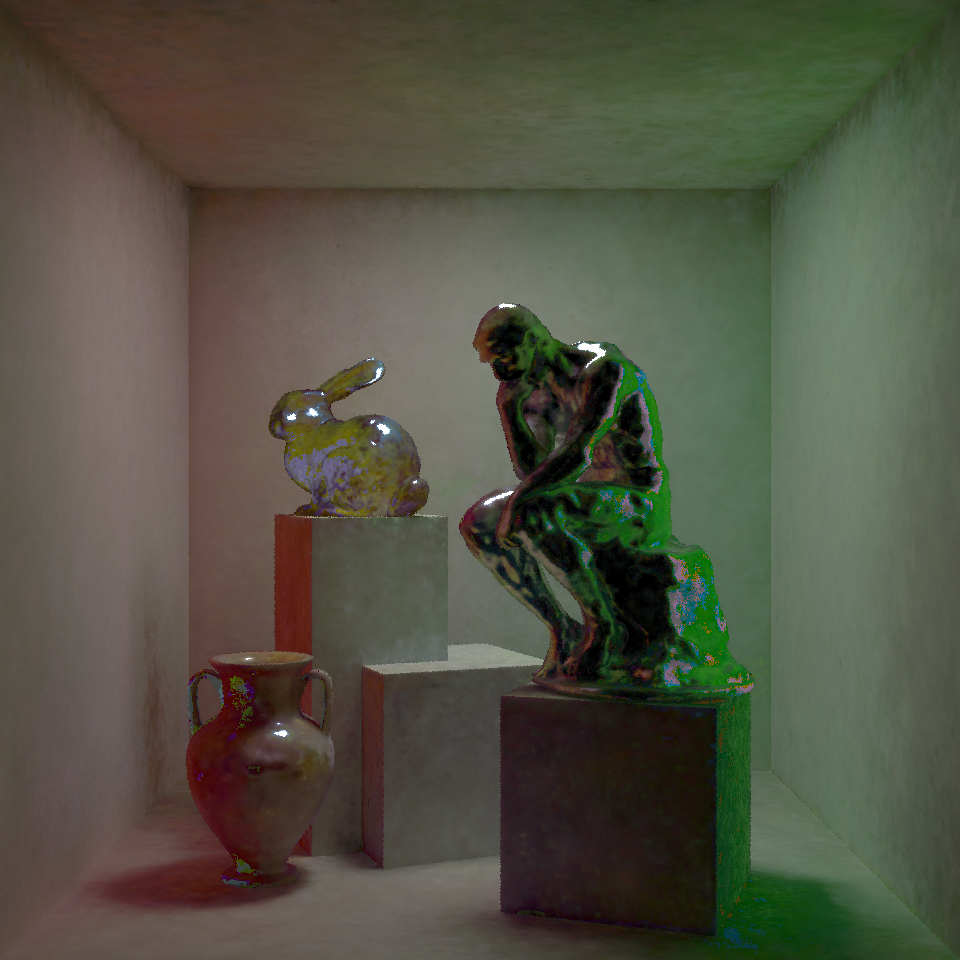
\includegraphics[width=0.8\linewidth]{py/tests/path_termination/rawcache_1spp_thinker.png}
    \end{subfigure}%
    \begin{subfigure}{0.3\textwidth}
        \centering
        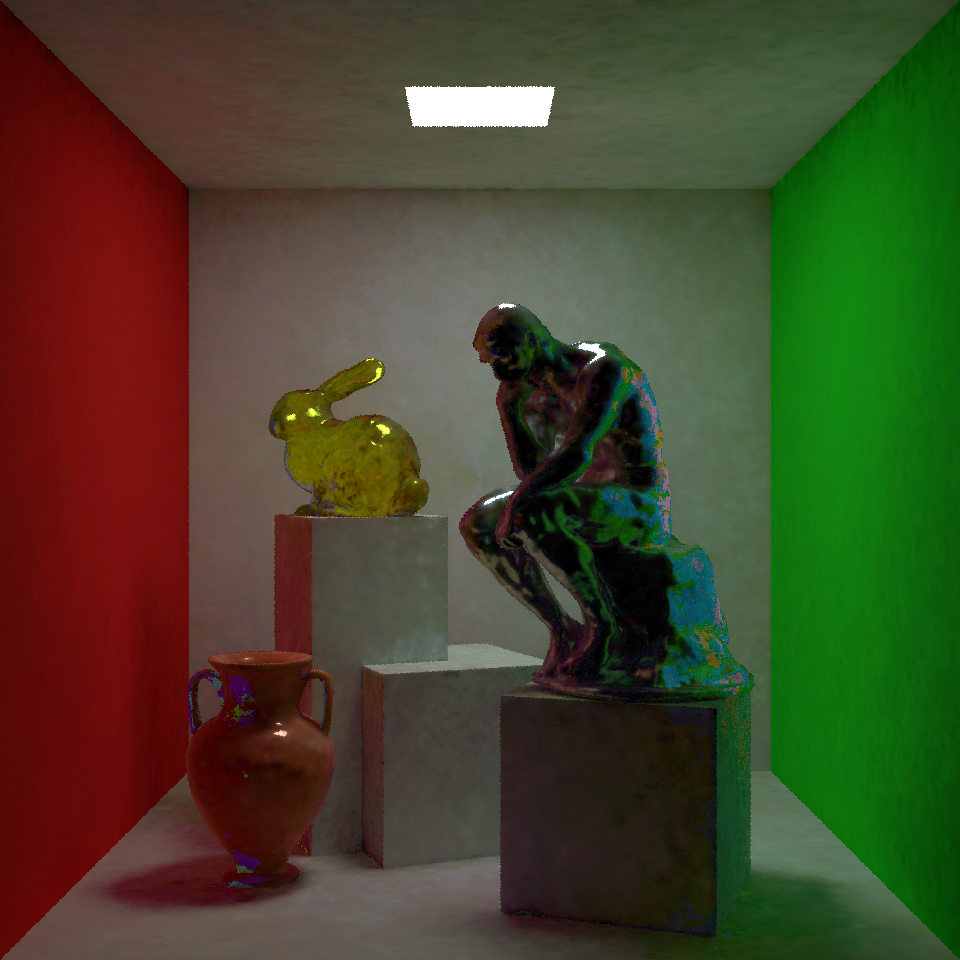
\includegraphics[width=0.8\linewidth]{py/tests/path_termination/1stvert_1spp_thinker.png}
    \end{subfigure}
    \caption{Visualization of emission and reflectance factorization. Left: The raw network prediction with emission and reflectance factored out. Right: The prediction multiplied with reflectance and emission added back in.}
    \label{fig:nrc_factorization}
\end{figure}

\subsection{Emission Factorization}
Besides the reflectance factorization, I choose to exclude the emission term from the Neural Radiance Cache and only learn the integral part of the outgoing radiance (see \cref{fig:nrc_factorization}):
\begin{equation}
    \widehat{L}(\vec{x}, \wo) = L_e(\vec{x}, \wo) + \left( \vec{F}_d(\vec{x}, \wo) + \vec{F}_s(\vec{x}, \wo) \right) \cdot \mathrm{NRC}(\vec{x}, \wo),
\end{equation}
This is because the emission term is usually magnitudes higher than the rest of the radiance field and only sparsely present, which leads to high variance in the training data and can lead to leaking of emission into other regions of the cache.
In addition, it does not affect performance, as the emission is directly given by the scene geometry, so we can simply add it during inference.

\section{Training}

\subsection{Collecting Training Data}
\begin{algorithm}
    \caption{Back transportation of radiance along the training paths}
    \label{alg:backtransport}
    \begin{algorithmic}
        \State $\vec{L}_T \gets \vec{L_e}$
        \For{$i \in (n - 1), \dots, 1$}
            \State $\vec{L}_T \gets w_i \cdot \vec{L}_T$ \Comment{Transport radiance to previous vertex}
            \State $\vec{L}_i \gets \vec{L}_i + \vec{L}_T$ \Comment{Accumulate radiance at vertex}
        \EndFor
    \end{algorithmic}
\end{algorithm}
\textcite{muller2021} combine the training data collection with the inference step by extending a fraction of the inference paths with additional training bounces to avoid redundant path tracing.
However, to enable mixing of different training techniques and to keep flexibility with the implementation, I chose to separate the training data collection from the inference step, accepting potential performance penalties.
Yet, \textcite{dereviannykh2024} even found performance benefits in this approach since it decreases incoherence.
Nevertheless, the training sample acquisition is the same:
First, trace paths from the camera to the scene, using Russian Roulette termination (\cref{eq:rr}) and Next Event Estimation (\cref{sec:mis}).
At each vertex of the path, store the current contribution weight and the input vector.
When sampling an emitter, these weights can then be used to transport the radiance back to the previous vertices (see \cref{alg:backtransport}).

To store the training data, a fixed-size ring buffer with an atomic counter is used to ensure thread safety.
This is not ideal, as it may lead to serialization of the GPU threads and thus potentially introduces a performance bottleneck, but it allows for writing dynamic amounts of data per thread.
Further research could be done to find a more efficient way to store the training data, for example using warp aggregation and compaction, but this is not straightforward as OptiX does not expose shared memory to allow for Shader Execution Reordering.

\subsection{Self-Learning}
Furthermore, \textcite{muller2021} propose a self-learning approach, which trades additional bias for reduced variance in the training data.
The idea is, to terminate the training paths into the radiance cache from the previous frame to simulate infinite length paths.
Because this can amplify the existing bias in the network prediction, they terminate $1/16$ of the training paths in an unbiased manner without self-learning but by Russian Roulette.

\subsection{Loss Function}
Because we use Monte Carlo Sampling to generate the training data, we want the network to learn the mean of the samples in a local region.
Furthermore, we assume the samples to be normally distributed by the central limit theorem, so the loss function should be the squared error loss (L2).

However, the network prediction may cover a high dynamic range, especially when the scene contains caustics or highly glossy materials.
The traditional L2 loss would thus disproportionately penalize losses in these regions, leading to possible overfitting on bright regions and bad representation of dark regions.
To mitigate this, \textcite{lehtinen2018} propose to normalize the L2 loss by the squared prediction of the network.
This thesis uses the modification of \textcite{muller2021}, who use the squared \emph{luminance} of the prediction instead for normalization to prevent overfitting onto individual color channels.

\section{Inference}
Using the described training process, the Neural Radiance Cache learns an approximation of the outgoing radiance field, denoted as $\widehat{L}(\vec{x}, \wo)$.
For inference, short paths are traced from the camera to the scene using BSDF sampling, the resulting contribution $I$ is then the throughput along the path multiplied with the radiance estimate at the terminal vertex.
The length of the inference paths is a trade-off between bias and variance, as longer paths can cover up cache inaccuracies but introduce Monte Carlo noise.
This is analogous to Final Gathering in Photon Mapping \parencite{jensen1996}.
In the following, I will thus discuss different strategies for path termination.

\subsection{Path Termination Strategies}
\label{sec:path_termination}
\paragraph{1st Vertex}
\label{par:pt_1st_vertex}
Terminating directly at the first path vertex is a simple strategy that is well suited to visualize the weaknesses of the radiance cache, but is a rather poor choice for glossy vertices that expose high frequency details in the radiance field.

\paragraph{1st Diffuse Vertex}
\label{par:pt_1st_diffuse}
For the aforementioned reasons, it can be beneficial to terminate at the first \emph{diffuse} vertex instead.
If a vertex is diffuse can be determined in the simplest case by the luminance of its diffuse albedo $\rho_d$.
This does not include the Fresnel effect however, thus a more sophisticated model could use the directional albedo $F_d$ or compare the importance sampling PDF $p(\wi)$ to the Lambertian PDF $p_d(\wi)$.
Yet, I found this approximation to be sufficient in practice.

\paragraph{Spread Angle Heuristic (SAH)}
\label{par:pt_sah}
\textcite{muller2021} propose to terminate paths instead based on the estimated spread of the sampled path.
Low spread paths should be path traced, because they exhibit high frequent detail and importance sampling these paths is likely to yield a good estimate.
High spread paths on the other hand result in high Monte Carlo noise but low-frequency details, making them suitable for interpolation through radiance caching.

\begin{figure}[htb!]
    \centering
    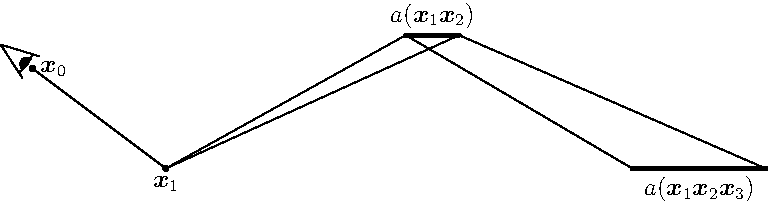
\includegraphics{asy/sah.pdf}
    \caption{The spread along a subpath is proportional to the path length and the inverse of the sampling PDF in solid angle measure, which is intuitively the solid angle covered by the sampled direction.}
    \label{fig:sah}
\end{figure}

\textcite{muller2021} use the findings from \textcite{bekaert2003}, according to which the isotropic spread of a subpath $\x_1 \cdots \x_n$ traced from the camera vertex $\x_0$ can be approximated as
\begin{equation}
    a(\x_1 \cdots \x_n) = \left(\sum_{k=2}^{n} \sqrt{\frac{\|\x_{k-1} - \x_k\|^2}{p(\wi_{k-1} \mid \wo_{k-1}) |\cos {\theta_o}_k|}}\right)^2,
\end{equation}
where $p(\wi_{k-1} \mid \wo_{k-1})$ is the importance sampling PDF of the current vertex in solid angle measure and ${\theta_o}_k$ is the incident angle at the current vertex.
Interestingly, as we will later see, the part under the square root is simply the inverse of the sampling PDF in surface area measure (\cref{eq:area_solid_angle_p}), so this term is an estimate for the covered area.
By taking the sum over the roots of areas, we are essentially summing the radii.
Squaring this sum thus gives us the area spread over the whole path (see \cref{fig:sah}).

To terminate paths, they compare the spread of the subpath to the spread at the primary vertex:
\begin{equation}
    a(\x_1 \cdots \x_n) > c \cdot a_0(\x_0), \quad a_0(\x_0) = \frac{\|\x_0 - \x_1\|}{4 \pi |\cos {\theta_o}_1|},
\end{equation}
where $c$ is a user-defined threshold and $4\pi$ is the area of a spherical image plane.
\textcite{muller2021} suggest $c=0.01$.
However, a limitation of this approach is that it will never terminate paths at the first vertex, because the spread is only defined for subpaths with $n \geq 2$.

\paragraph{Balanced Termination Heuristic (BTH)}
\label{par:pt_bth}
\textcite{dereviannykh2024} propose combining SAH with a stochastic path termination strategy based on the balance heuristic (\cref{eq:balance_heuristic}) for more aggressive termination already at the first vertex.
They define the continuation probability by calculating the MIS weight against a factor $1/\pi$ per NIRC sample.
Instead, I propose to use the power heuristic with $\beta=2$ against the Lambertian diffuse PDF $p_d(\wi)$:
\begin{equation}
    p_{\text{continue}}(\wi) = \frac{p(\wi \mid \wo)^\beta}{p(\wi \mid \wo)^\beta + K p_d(\wi)^\beta}
\end{equation}
This way the continuation probability will be exactly $1/(K+1)$ if the surface is diffuse, giving an intuitive control over the termination probability.

\subsection{Temporal Stability}
Because the neural network is trained continuously with a relatively high learning rate on highly dynamic data, the output of the network can become temporally unstable.
As a solution to this apparent flickering effect, \textcite{muller2021} propose to use an exponential moving average over the network weights for inference.
Note, however, that this is used exclusively for inference, leaving the training process unchanged.